%%%%%%%%%%%%  Generated using docx2latex.com  %%%%%%%%%%%%%%

%%%%%%%%%%%%  v2.0.0-beta  %%%%%%%%%%%%%%

\documentclass[12pt]{report}
\usepackage{amsmath}
\usepackage{latexsym}
\usepackage{amsfonts}
\usepackage[normalem]{ulem}
\usepackage{soul}
\usepackage{array}
\usepackage{amssymb}
\usepackage{extarrows}
\usepackage{graphicx}
\usepackage[backend=biber,
style=numeric,
sorting=none,
isbn=false,
doi=false,
url=false,
]{biblatex}\addbibresource{bibliography.bib}

\usepackage{subfig}
\usepackage{wrapfig}
\usepackage{wasysym}
\usepackage{enumitem}
\usepackage{adjustbox}
\usepackage{ragged2e}
\usepackage[svgnames,table]{xcolor}
\usepackage{tikz}
\usepackage{longtable}
\usepackage{changepage}
\usepackage{setspace}
\usepackage{hhline}
\usepackage{multicol}
\usepackage{tabto}
\usepackage{float}
\usepackage{multirow}
\usepackage{makecell}
\usepackage{fancyhdr}
\usepackage[toc,page]{appendix}
\usepackage[hidelinks]{hyperref}
\usetikzlibrary{shapes.symbols,shapes.geometric,shadows,arrows.meta}
\tikzset{>={Latex[width=1.5mm,length=2mm]}}
\usepackage{flowchart}\usepackage[paperheight=11.69in,paperwidth=8.27in,left=0.5in,right=0.5in,top=0.5in,bottom=0.5in,headheight=1in]{geometry}
\usepackage[utf8]{inputenc}
\usepackage[T1]{fontenc}
\TabPositions{0.5in,1.0in,1.5in,2.0in,2.5in,3.0in,3.5in,4.0in,4.5in,5.0in,5.5in,6.0in,6.5in,7.0in,}

\urlstyle{same}

\renewcommand{\_}{\kern-1.5pt\textunderscore\kern-1.5pt}

 %%%%%%%%%%%%  Set Depths for Sections  %%%%%%%%%%%%%%

% 1) Section
% 1.1) SubSection
% 1.1.1) SubSubSection
% 1.1.1.1) Paragraph
% 1.1.1.1.1) Subparagraph


\setcounter{tocdepth}{5}
\setcounter{secnumdepth}{5}


 %%%%%%%%%%%%  Set Depths for Nested Lists created by \begin{enumerate}  %%%%%%%%%%%%%%


\setlistdepth{9}
\renewlist{enumerate}{enumerate}{9}
		\setlist[enumerate,1]{label=\arabic*)}
		\setlist[enumerate,2]{label=\alph*)}
		\setlist[enumerate,3]{label=(\roman*)}
		\setlist[enumerate,4]{label=(\arabic*)}
		\setlist[enumerate,5]{label=(\Alph*)}
		\setlist[enumerate,6]{label=(\Roman*)}
		\setlist[enumerate,7]{label=\arabic*}
		\setlist[enumerate,8]{label=\alph*}
		\setlist[enumerate,9]{label=\roman*}

\renewlist{itemize}{itemize}{9}
		\setlist[itemize]{label=$\cdot$}
		\setlist[itemize,1]{label=\textbullet}
		\setlist[itemize,2]{label=$\circ$}
		\setlist[itemize,3]{label=$\ast$}
		\setlist[itemize,4]{label=$\dagger$}
		\setlist[itemize,5]{label=$\triangleright$}
		\setlist[itemize,6]{label=$\bigstar$}
		\setlist[itemize,7]{label=$\blacklozenge$}
		\setlist[itemize,8]{label=$\prime$}



 %%%%%%%%%%%%  Header here  %%%%%%%%%%%%%%


\pagestyle{fancy}
\fancyhf{}
\cfoot{ 
\vspace{\baselineskip}

\vspace{\baselineskip}
}
\renewcommand{\headrulewidth}{0pt}
\setlength{\topsep}{0pt}\setlength{\parskip}{9.96pt}
\setlength{\parindent}{0pt}

 %%%%%%%%%%%%  This sets linespacing (verticle gap between Lines) Default=1 %%%%%%%%%%%%%%


\renewcommand{\arraystretch}{1.3}


%%%%%%%%%%%%%%%%%%%% Document code starts here %%%%%%%%%%%%%%%%%%%%



\begin{document}


 %%%%%%%%%%%%  This Produces Table Of Contents %%%%%%%%%%%%%%

\tableofcontents
\addcontentsline{toc}{chapter}{Contents}

\vspace{\baselineskip}

\vspace{\baselineskip}
\section*{Prob: Set theory }
\addcontentsline{toc}{section}{Prob: Set theory }
\subsection*{Basic}
\addcontentsline{toc}{subsection}{Basic}
\begin{itemize}
	\item \textbf{Set} is a collection of well-defined objects (called elements or members): x  A.\par

	\item Set can be represented by a list, i.e. A = $ \{ $ -2, 2$ \} $ , or by a set-builder, i.e. A = $ \{ $ x $ \vert $  x\textsuperscript{2}\textsubscript{ }– 4 = 0$ \} $ .\par

	\item The \textbf{cardinality} of the set is the number of elements in that set $\#$ (A), a set can be finite set or infinite set, a set can be countable or uncountable.\par

	\item A \textbf{subset} of a set: A  B if any element of A is also an element of B; apparently   A  A. \par

	\item If A  B and A  B we have A  B.\par

	\item Absolute \textbf{complement} of A: A\textsuperscript{c} = $ \{ $ x $ \vert $  x  A$ \} $ \par

	\item Relative complement of A with respect to B: B – A = $ \{ $ x $ \vert $  x  B and x  A$ \} $ \par

	\item \textbf{Union}: A  B = $ \{ $ x $ \vert $  x  A or x  B$ \} $ ; this relation can be extended to more than two sets.\par

	\item \textbf{Intersection}: A  B = $ \{ $ x $ \vert $  x  A and x  B$ \} $ ; again, this can be extended.\par

	\item If\  A  B = , A and B are \textbf{disjoint} sets. \ \ \  \par


\end{itemize}\subsection*{Intermediate}
\addcontentsline{toc}{subsection}{Intermediate}
\begin{itemize}
	\item Three basic laws of sets and De Morgan’s laws\par

\begin{itemize}
	\item \textbf{Commutative} \tab A  B = B  A; \tab \tab \tab \tab and A  B = B  A\par

	\item \textbf{Associative} \tab A  (B  C) = (A  B)  C; \tab \tab and A  (B  C) = (A  B)  C\par

	\item \textbf{Distributive} \tab A  (B  C) = (A  B)  (A  C); \tab and A  (B  C) = (A  B)  (A  C)\par

	\item \textbf{De} \textbf{Morgan} \tab (A  B)\textsuperscript{c} = A\textsuperscript{c}  B\textsuperscript{c}; \tab \tab \tab and (A  B)\textsuperscript{c} = A\textsuperscript{c}  B\textsuperscript{c}\par

(De Morgan’s law can be extended to more than two sets)\par


\end{itemize}
	\item \textbf{Inclusion-Exclusion principles}: suppose that A and B are finite sets, then:\par

\begin{itemize}
	\item If A  B, $\#$ (A) $ \leq $  $\#$ (B)\par

	\item $\#$ (A  B) = $\#$ (A) + $\#$ (B) - $\#$ (A  B)\par

	\item Extension: $\#$ (A  B  C) = $\#$ (A) + $\#$ (B) + $\#$ (C) - $\#$ (A  B) - $\#$ (B  C) - $\#$ (C  A) + $\#$ (A  B  C)\par


\end{itemize}
	\item Cartesian product\par

\begin{itemize}
	\item A \textbf{Cartesian product} of two sets A, B is the set A $ \times $  B = $ \{ $ (a,b) $ \vert $  a  A and b  B$ \} $ \par

	\item $\#$ (A $ \times $  B) = $\#$ (A) $\#$ (B)\par


\end{itemize}
\end{itemize}\section*{Prob: Permutation and Combination}
\addcontentsline{toc}{section}{Prob: Permutation and Combination}
\begin{itemize}
	\item Fundamental \textbf{principle of counting}: if a choice consists of k steps, each step i can be made in n\textsubscript{i} ways, the whole choice can be made in n\textsubscript{1}  n\textsubscript{2}  n\textsubscript{k} ways.\par

	\item Permutation: a permutation is an\textbf{ ordered arrangement} of objects. The number of permutation of n objects is n  (n-1)  (n-2)  1 = n! (0! = 1)\par

	\item Permutations of a set of distinct objects taken from a larger set: suppose we have n items, the number of ordered arrangement of k items can we from these n items is \textbf{\textsubscript{n}P\textsubscript{k}} = n! / (n-k)!  \par

	\item Combination is a possible selection of a certain number of objects taken from a group \textbf{without regard to order}. The number of k-element subset of an n-element set is \textbf{\textsubscript{n}C\textsubscript{k}} = \textbf{\textsubscript{n}P\textsubscript{k}} / k! = n! / (k!$\ast$ (n-k)!). Alternative not. (n k)\par

	\item Properties:\par

\begin{itemize}
	\item Symmetry\tab \tab  \( C_{k}^{n}=C_{n-k}^{n} \) \par

	\item Pascal \tab \tab \tab  \( C_{k}^{n+1}=C_{k-1}^{n}+C_{k}^{n} \) \par

	\item Binomial theorem\tab  \(  \left( x+y \right) ^{n}= \sum _{k=0}^{n}C_{k}^{n}x^{n-k}y^{k} \)  (proof by induction)
\end{itemize}
\end{itemize}\par

\begin{adjustwidth}{1.0in}{0.0in}
Application: number of subsets of a set with n elements  \(  \sum _{k=0}^{n}C_{k}^{n}= \left( 1+1 \right) ^{n}=2^{n} \) \par

\end{adjustwidth}

\begin{itemize}
	\item Combination with \textbf{repetition}: count the way to select k objects from n different categories with repetition allowed  pictorially convert to k \textbf{\textit{stars}} and n-1 \textbf{\textit{bars}}  problem of insert k stars into k+n-1 position:  \( C_{k}^{k+n-1} \) \par

	\item Permutation with \textbf{indistinguishable} objects (\textbf{partition}): suppose we have n objects where n\textsubscript{1} of them are identical, n\textsubscript{2} of them are identical$ \ldots $  and n\textsubscript{k} of them are identical and n\textsubscript{1} + n\textsubscript{2} + ... + n\textsubscript{k} = n. The number of permutation of n objects are then  \( \frac{n!}{n_{1}! \cdot n_{2}! \cdot  \cdot  \cdot n_{k}!} \) .
\end{itemize}\par

\section*{Prob: Probability}
\addcontentsline{toc}{section}{Prob: Probability}
\subsection*{Basic}
\addcontentsline{toc}{subsection}{Basic}
\begin{itemize}
	\item A (random) \textbf{experiment} is a process whose \textbf{outcomes} cannot be predicted with certainty. \par

	\item The \textbf{sample space} S of an experiment is the set of all possible outcomes.\par

	\item An \textbf{event} E is a subset of the sample space.\par

	\item \textbf{Probability} is the measure of occurrence of an event.\par

\begin{itemize}
	\item Experimental probability uses the relative frequency $\&$  the law of large numbers (n is $\#$  of experiments)\par

 \[ P \left( E \right) =\mathop{\lim }_{n \rightarrow \infty}\frac{\# \left( E \right) }{n} \] \par

	\item Theoretical or classical probability applies \textbf{only when all possible outcomes are} \textbf{equally likely}
\end{itemize}
\end{itemize}\par

\begin{adjustwidth}{1.0in}{0.0in}
 \[ P \left( E \right) =\frac{\# \left( E \right) }{\# \left( S \right) } \] \par

\end{adjustwidth}

\begin{itemize}
	\item Any function P satisfies the following axioms (\textbf{Kolmogorov} axioms) can be a \textbf{probability} measure.\par

\begin{itemize}
	\item For any event E,  \( 0 \leq P \left( E \right)  \leq 1 \) .  \( P \left( S \right) =1 \) \par

	\item For any sequence of mutually exclusive events $ \{ $ E\textsubscript{n$ \geq $ 1}$ \} $  and Ei  Ej =  for i  j, we have\par

 \[ P \left(  \bigcup_{n=1}^{\infty}E_{n} \right) = \sum _{n=1}^{\infty}P \left( E_{n} \right)  \] \par


\end{itemize}
	\item If P is a probability measure, then\par

\begin{itemize}
	\item If $ \{ $ E1, E2, $ \ldots $ , En$ \} $  is a finite set of mutually exclusive events then \par

 \[ P \left(  \bigcup_{k=1}^{n}E_{k} \right) = \sum _{n=1}^{\infty}P \left( E_{n} \right)  \] \par

	\item P(E\textsuperscript{c}) = 1 – P(E)\par

	\item If events A and B are mutually exclusive (sets A and B are disjoint): P(A  B) = P() = 0 \par

	\item If A  B then P(A) $ \leq $  P(B)\par

	\item With events A and B: P(A  B) = P(A) + P(B) – P(A  B) \par

Extension: P(A B  C) = P(A) + P(B) + P(C) – P(A  B) – P(B  C) – P(C  A) + P(A  B  C)\par

Extension: A = A  (B  B\textsuperscript{c}) = (A  B)  (A  B\textsuperscript{c})  P(A) = P(A  B) + P(A  B\textsuperscript{c})\par


\end{itemize}
\end{itemize}\subsection*{Conditional probability and Bayes’s formula}
\addcontentsline{toc}{subsection}{Conditional probability and Bayes’s formula}
\begin{itemize}
	\item Conditional probability: \par

\begin{itemize}
	\item Basic: if the occurrence of event A depends on the occurrence of B then the probability of A given B provided that P(B)  0, denoted as P(A$ \vert $ B), is:\par

 \[ P \left( A \vert B \right) =\frac{\# \left( A \cap B \right) }{\# \left( B \right) }=\frac{P \left( A \cap B \right) }{P \left( B \right) } \] \par

\tab Extension: P(A) = P(A$ \vert $ B)P(B) + P(A$ \vert $ B\textsuperscript{c})P(B\textsuperscript{c})\par

\tab Extension: P(B\textsuperscript{c}$ \vert $ A) = 1 – P(B$ \vert $ A)\par

	\item Generalization of the basic formula\par

 \[ P \left( A_{1} \cap A_{2} \cap A_{3} \ldots  \right) =P \left( A_{1} \right) +P \left( A_{2} \vert A_{1} \right) +P \left( A_{3} \vert A_{1} \cap A_{2} \right) + \ldots  \] \par


\end{itemize}
	\item Bayes’s formula\par

\begin{itemize}
	\item \textbf{Theorem}: since  \( P \left( A \cap B \right) =P \left( B \cap A \right)  \)  hence  \( P \left( A \vert B \right)  \cdot P \left( B \right) =P \left( B \vert A \right)  \cdot P \left( A \right)  \) , we have:\par

 \[ P \left( B \vert A \right) =\frac{P \left( A \vert B \right)  \cdot P \left( B \right) }{P \left( A \right) } \] \par

	\item Extension:  \( P \left( B \vert A \right) =\frac{P \left( A \cap B \right) }{P \left( A \cap B \right) +P \left( A \cap B^{c} \right) }=\frac{P \left( A \vert B \right)  \cdot P \left( B \right) }{P \left( A \vert B \right)  \cdot P \left( B \right) +P \left( A \vert B^{c} \right)  \cdot P \left( B^{c} \right) } \) \par

	\item \textbf{Law of Total probability}: suppose that the sample space S is the union of mutually exclusive events H\textsubscript{1}, H\textsubscript{2}, $ \ldots $ , H\textsubscript{n} with P(H\textsubscript{i}) > 0. Then for any event A we have:\par

 \[ P \left( A \right) =P \left( A \cap H_{1} \right) +P \left( A \cap H_{2} \right) + \ldots =P \left( A \vert H_{1} \right)  \cdot P \left( H_{1} \right) +P \left( A \vert H_{2} \right)  \cdot P \left( H_{2} \right) + \ldots  \] \par

	\item \textbf{Generalization of Bayes’s rule}\par

 \[ P \left( H_{i} \vert A \right) =\frac{P \left( A \vert H_{i} \right)  \cdot P \left( H_{i} \right) }{P \left( A \right) } \] \par

in which P(A) = P(H\textsubscript{1})P(A$ \vert $ H\textsubscript{1}) + P(H\textsubscript{2})P(A$ \vert $ H\textsubscript{2}) + $ \ldots $  + P(H\textsubscript{n})P(A$ \vert $ H\textsubscript{n})\par

	\item \textbf{Prior probability}: the \textbf{unconditional probability} P(A) is the probability of the event A prior to introducing new events that may affect A. \par

	\item \textbf{Posterior probability}: when the occurrence of an event B will affect event A, the \textbf{conditional probability} P(A$ \vert $ B) is known as the posterior probability of A. \par


\end{itemize}
	\item Independent events\par

\begin{itemize}
	\item In term of conditional probability, two events A and B are said to be \textbf{independent} if and only if:\par

 \[ P \left( A \vert B \right) =P \left( A \right)  \] \par

	\item General, A and B are independent events if and only if:\par

 \[ P \left( A \cap B \right) =P \left( A \right)  \cdot P \left( B \right)  \] \par

	\item If A and B are independent, then so A and B\textsuperscript{c}; A\textsuperscript{c} and B\textsuperscript{c}.\par

	\item Events A\textsubscript{1}, A\textsubscript{2}, $ \ldots $ , A\textsubscript{n} are said to be independent if for any 1 $ \leq $  i\textsubscript{1} < i\textsubscript{2} < $ \ldots $  < i\textsubscript{k} $ \leq $  n we have: \par

 \[ P \left( A_{i1} \cap A_{i2} \cap  \ldots  \cap A_{ik} \right) =P \left( A_{i1} \right)  \cdot P \left( A_{i2} \right)  \cdot  \ldots  \cdot P \left( A_{ik} \right)  \] \par

	\item Conditionally independent: two events A and B are said to be conditionally independent, given another event C with P(C) > 0, if:
\end{itemize}
\end{itemize}\par

\begin{adjustwidth}{1.0in}{0.0in}
 \[ P \left( A \cap B \vert C \right) =P \left( A \vert C \right)  \cdot P \left( B \vert C \right)  \] \par

\end{adjustwidth}

\begin{adjustwidth}{1.0in}{0.0in}
If P(B  C) > 0, conditional independence is equivalent to:\par

\end{adjustwidth}

\begin{adjustwidth}{1.0in}{0.0in}
 \[ P \left( A \vert B \cap C \right) =P \left( A \vert C \right)  \] \par

\end{adjustwidth}

\begin{itemize}
	\item Odds and conditional probability\par

\begin{itemize}
	\item If E is the event of all \textbf{favorable outcomes,} then E\textsuperscript{c} is the event of \textbf{unfavorable outcomes}. Hence:\par

 \[ \mathrm{\text{odds in favor}}=\frac{\# \left( E \right) }{\# \left( E^{c} \right) };~~~\mathrm{\text{odds against}}=\frac{\# \left( E^{c} \right) }{\# \left( E \right) } \] \par

Consequently:\par

 \[ P \left( E \right) =\frac{\# \left( E \right) }{\# \left( E \right) +\# \left( E^{c} \right) }\text{;~~ P} \left( E^{c} \right) =\frac{\# \left( E^{c} \right) }{\# \left( E \right) +\# \left( E^{c} \right) } \] \par

 \[ \mathrm{\text{odds in favor}}=\frac{P \left( E \right) }{1-P \left( E \right) };~~~\mathrm{\text{odds against}}=\frac{1-P \left( E \right) }{P \left( E \right) } \] \par


\end{itemize}
\end{itemize}\section*{Prob: Random variables}
\addcontentsline{toc}{section}{Prob: Random variables}
\subsection*{Basis}
\addcontentsline{toc}{subsection}{Basis}
\begin{itemize}
	\item \textbf{Random variable}: is a function with domain the sample space and range a subset of real numbers, notation X(s) = x means x is the value associated with the outcome s by the random variable X. \par

	\item Notation:\par

\begin{itemize}
	\item X, Y, Z are random variables; x, y, z are possible values that the X, Y, Z random variables can take;\par

	\item The statement $``$X = x$"$  defines an event consisting of all outcomes with X-measurement equal to x;\par

	\item P(X = x) is then the probability of the event X = x.\par


\end{itemize}
	\item Type of random variables:\par

\begin{itemize}
	\item \textbf{Discrete}: a random variable whose range is either finite or countably infinite;\par

	\item \textbf{Continuous}: a random variable whose range is an interval in ;\par

	\item \textbf{Mixed}: partially discrete and partially continuous.\par


\end{itemize}
\end{itemize}\subsection*{Properties}
\addcontentsline{toc}{subsection}{Properties}
\begin{itemize}
	\item All random variables (discrete, continuous, mixed) have a distribution function or a cumulative distribution function (cdf). If X is a random variable then the cumulative distribution function, is the function:\par

 \[ F \left( x \right) =P \left( X \leq x \right)  \] \par

and, hence: \par

 \[ P \left( X>a \right) =1-F \left( a \right)  \] \par

Any non-negative function satisfying the three following propositions can be a cdf:\par

\begin{itemize}
	\item If a $ \leq $  b then F(a) $ \leq $  F(b)\par

	\item  \( \mathop{\lim }_{a \rightarrow +b}F \left( a \right) =F \left( b \right)  \) \par

	\item  \( \mathop{\lim }_{a \rightarrow -\infty}F \left( a \right) =0;~ \mathop{\lim }_{a \rightarrow \infty}F \left( a \right) =1 \) 
\end{itemize}\par

\begin{adjustwidth}{0.5in}{0.0in}
Further properties: if a < b then\par

\end{adjustwidth}

\begin{itemize}
	\item P(a < X $ \leq $  b) = F(b) - F(a)\par

	\item P(a $ \leq $  X < b) = F(b\textsuperscript{-}) - F(a\textsuperscript{-})\par

	\item P(a $ \leq $  X $ \leq $  b) = F(b) - F(a\textsuperscript{-})  P(X = a) = F(a) - F(a\textsuperscript{-})\par

	\item P(a < X < b) = F(b\textsuperscript{-}) - F(a)
\end{itemize}\par

\begin{adjustwidth}{0.5in}{0.0in}
Type of graphs:\par

\end{adjustwidth}

\begin{itemize}
	\item For a continuous distribution, the graph of cdf is continuous non-decreasing curve. \par

	\item For a discrete distribution, the graph of its cdf consists of a series of horizontal lines with jumps between them. \par

	\item A cdf of a mixed distribution contains both jumps and pieces of continuous increasing curves.
\end{itemize}\par

	\item Survival distribution function (sdf), a.k.a. reliability function, gives the probability that an object of interest will survive beyond any given specified time. \par

 \[ S \left( x \right) =P \left( X>x \right) =1-P \left( X \leq x \right) =1-F \left( x \right)  \] \par

An example for the application of the survival distribution function: if a < b then\par

 \[ P \left( a<X \leq b \right) =F \left( b \right) -F \left( a \right) =S \left( a \right) - \left( b \right)  \] \par

Noted: for a continuous random variable, P(X = a) = F(a) - F(a\textsuperscript{-}) = 0  P(X $ \leq $  a) = P(X < a) + P(X = a) = P(X < a); finally we have: \par

 \[ P \left( X<a \right) =P \left( X \leq a \right) =F \left( a \right) =1-S \left( a \right)  \] \par


\end{itemize}\section*{Prob: (single) Discrete random variables}
\addcontentsline{toc}{section}{Prob: (single) Discrete random variables}
\subsection*{Basis}
\addcontentsline{toc}{subsection}{Basis}
\begin{itemize}
	\item \textbf{Discrete random variable} is a random variable whose range is either finite or countably infinite.\par

	\item \textbf{Probability mass function} (\textbf{pmf}) or \textbf{probability distribution} of a discrete random variable X:\par

\begin{itemize}
	\item p(x) = P(X = x): pmf gives the probability that a discrete random variable is \textbf{exactly equal} to some value.\par

	\item pmf can be an equation, a table or a graph.\par


\end{itemize}
	\item \textbf{Cumulative distribution function} (\textbf{cdf}) is a function giving the probability that the random variable X is \textbf{less than or equal to} x, for every value of x. For a discrete random variable:\par

\begin{itemize}
	\item Definition: cdf is found by \textbf{summing up} the probabilities:\par

 \[ F \left( a \right) =P \left( X \leq a \right) = \sum _{x \leq a}^{}p \left( x \right)  \] \par

	\item Extension: if the range of a discrete random variable X consists of the value x\textsubscript{1} < x\textsubscript{2} < $ \ldots $  < x\textsubscript{n} then: (1) p(x\textsubscript{1}) = F(x\textsubscript{1}), and (2) p(x\textsubscript{i}) = F(x\textsubscript{i}) – F(x\textsubscript{i-1}) for i = 2, 3, $ \ldots $ , n.\par


\end{itemize}
	\item \textbf{Expected value} (\textbf{mean value}) of a discrete random variable: let the range of a discrete random variable X be a sequence of number x\textsubscript{1}, x\textsubscript{2}, $ \ldots $ , x\textsubscript{k} and let p(x) be the corresponding probability mass function, then the expected value of X is:\par

 \[ E \left( X \right) = \sum _{i=1}^{k}x_{i}p \left( x_{i} \right)  \] \par

The expected value (or mean) is related to the physical property of \textbf{center of mass}. \par

	\item \textbf{Expected value} of a function of a discrete random variable\par

\begin{itemize}
	\item Definition: if X is a discrete random variable with range D and pmf p(x), then the expected value of the random variable g(X) is:\par

 \[ E \left( g \left( X \right)  \right) = \sum _{x \in D}^{}g \left( x \right)  \cdot p \left( x \right)  \] \par

\tab \tab where g:    is a real function.\par

	\item Extension: if X is a discrete random variable, then for any constants a and b, we have:\par

 \[ E \left( aX+b \right) =a \cdot E \left( X \right) +b \] \par

 \[ E \left( aX^{2}+bX+c \right) =a \cdot  E \left( X^{2} \right) +b \cdot E \left( X \right) +c \] \par

	\item Extension: if  \( g \left( x \right) =x^{n} \)  then we call  \( E \left( x^{n} \right) = \sum _{x}^{}x^{n} \cdot p \left( x \right)  \)  the n\textsuperscript{th}-moment about the origin of X, or the n\textsuperscript{th}-raw moment. Apparently,  \( E \left( X \right)  \)  is the first moment of X. \par


\end{itemize}
	\item \textbf{Variance} and \textbf{standard deviation} of a discrete random variable\par

\begin{itemize}
	\item Meaning: standard deviation measures how\textbf{ spread out} the \textbf{pmf} is about its\textbf{ expected value}\par

	\item \textbf{Variance}: the expected square distance between the random variable and its mean\par

	\item \textbf{Standard deviation}: the positive square root of the variance\par

 \[ \mathrm{Var} \left( X \right) = \sigma _{X}^{2}=E \left[  \left( X-E \left( X \right)  \right) ^{2} \right] =E \left( X^{2} \right) - \left( E \left( X \right)  \right) ^{2} \] \par

Extension:\par

 \[ \mathrm{Var} \left( X \right) =E \left( X \right) +E \left( X \cdot  \left( X-1 \right)  \right) - \left( E \left( X \right)  \right) ^{2} \] \par

 \[ \mathrm{Var} \left( aX+b \right) =a^{2}\mathrm{  \cdot  Var} \left( X \right)  \] \par

	\item \textbf{Coefficient of variation }of a random variable X is defined as:\par

 \[ \mathrm{CV} \left( X \right) =\frac{ \sigma _{X}}{E \left( X \right) } \] \par


\end{itemize}
\end{itemize}\subsection*{Uniform discrete random variable}
\addcontentsline{toc}{subsection}{Uniform discrete random variable}
\begin{itemize}
	\item \textbf{[Commonly used]} Uniform discrete random variable\par

\begin{itemize}
	\item Definition: let X be a discrete random variable defined on a sample space S with n elements $ \{ $ x\textsubscript{1}, x\textsubscript{2}, $ \ldots $ , x\textsubscript{n}$ \} $ , and the pmf of X is\par

 \[ p \left( x_{i} \right) =\frac{1}{n}\mathrm{~~for~~}i=1, 2, \ldots ,n \] \par

	\item Properties: the expected value of X is\par

 \[ E \left( X \right) = \sum _{i=1}^{k}x_{i}p \left( x_{i} \right) =\frac{x_{1}+x_{2}+ \ldots +x_{n}}{n} \] \par

The second moment of X is\par

 \[ E \left( X^{2} \right) = \sum _{i=1}^{k}x_{i}^{2}p \left( x_{i} \right) =\frac{x_{1}^{2}+x_{2}^{2}+ \ldots +x_{n}^{2}}{n} \] \par

\tab The variance of X is \par

 \[ \mathrm{Var} \left( X \right) =E \left( X^{2} \right) - \left( E \left( X \right)  \right) ^{2}=\frac{x_{1}^{2}+x_{2}^{2}+ \ldots +x_{n}^{2}}{n}-\frac{ \left( x_{1}+x_{2}+ \ldots +x_{n} \right) ^{2}}{n} \] \par

	\item In case if x = $ \{ $ a, a + h, a + 2$\ast$ h, ..., a + (n-1)$\ast$ h$ \} $  then we have:\par

 \[ E \left( X \right) =a+\frac{h \cdot  \left( n-1 \right) }{2} \] \par

 \[ E \left( X^{2} \right) =a^{2}+ah \cdot  \left( n-1 \right) +h^{2}\frac{ \left( n-1 \right)  \left( 2n-1 \right) }{6} \] \par

 \[ \mathrm{Var} \left( X \right) =E \left( X^{2} \right) - \left( E \left( X \right)  \right) ^{2}=\frac{h^{2} \cdot  \left( n^{2}-1 \right) }{12} \] \par

	\item In case if x = $ \{ $ a, a + 1, a + 2, ..., b$ \} $  then we have:\par

 \[ p \left( x_{i} \right) =\frac{1}{b-a+1} \] \par

 \[ E \left( X \right) =\frac{a+b}{2} \] \par

 \[ E \left( X^{2} \right) =ab+\frac{ \left( b-a \right)  \left( 2b-2a+1 \right) }{6} \] \par

 \[ \mathrm{Var} \left( X \right) =E \left( X^{2} \right) - \left( E \left( X \right)  \right) ^{2}=\frac{ \left( b-a+1 \right) ^{2}-1}{12} \] \par

 \[ M_{X} \left( t \right) =E \left( e^{tX} \right) = \sum _{x=0}^{b-a}e^{t \left( x+a \right) } \cdot p \left( x+a \right) =\frac{e^{ta}}{b-a+1} \left( \frac{1-e^{t \left( b-a+1 \right) }}{1-e^{t}} \right)  \] \par


\end{itemize}
\end{itemize}\subsection*{Binomial random variable}
\addcontentsline{toc}{subsection}{Binomial random variable}
\begin{itemize}
	\item \textbf{[Commonly used]} Binomial random variable\par

\begin{itemize}
	\item Background: a \textbf{Bernoulli trial }is an experiment with\textbf{ exactly two outcomes: success and failure} with the corresponding \textbf{probability of p and q}. Moreover: 0 < p, q < 1 and \textbf{p + q = 1} (e.g. flips of a coin). A \textbf{Bernoulli experiment} is a sequence of independent Bernoulli trials. \par

Let X represent the\textbf{ number of success} that occur in \textbf{n independent Bernoulli trials}, then X is said to be a \textbf{binomial random variable} with parameters \textbf{(n,p)}. If n = 1 then X is a \textbf{Bernoulli random variable}. The main problem of a binomial experiment is to find the \textbf{probability of r success out of n trials}. \par

	\item The probability of having r successes out of n trials\textbf{ in any order} is given by the \textbf{binomial mass function}:\par

 \[ p \left( r \right) =P \left( X=r \right) = \left( \begin{matrix}
n\\
r\\
\end{matrix}
 \right) p^{r}q^{n-r} \] \par

Note that as q = 1 – p: \par

 \[  \sum _{k=0}^{n}p \left( k \right) = \sum _{k=0}^{n} \left( \begin{matrix}
n\\
k\\
\end{matrix}
 \right) p^{k} \left( 1-p \right) ^{n-k}= \left( p+1-p \right) ^{n}=1 \] \par

 \[ p \left( r \right) =\frac{p}{1-p} \times \frac{n-r+1}{r} \times p \left( r-1 \right)  \] \par

From the above formula, it is proven that  \( p \left( r \right)  \)  has a unique global maximum at  \( r= \lfloor  \left( n+1 \right)  \cdot p \rfloor  \)  (and  \(  \left( n+1 \right)  \cdot p-1 \)  if  \(  \left( n+1 \right)  \cdot p \)  is an integer).\par

	\item The cumulative distribution function is given by:\par

 \[ F \left( x \right) =P \left( X \leq x \right) = \left\{ \begin{matrix}
0  &  x<0\\
 \sum _{k=0}^{ \lfloor x \rfloor } \left( \begin{matrix}
n\\
k\\
\end{matrix}
 \right) p^{k} \left( 1-p \right) ^{n-k}  &  0 \leq x \leq n\\
1  &  x>n\\
\end{matrix}
  \] \par

where  \(  \lfloor x \rfloor  \)  is the floor function.\par

	\item The expected value of the binomial distribution is given by:\par

 \[ E \left( X \right) = \sum _{k=1}^{n}k \left( \begin{matrix}
n\\
k\\
\end{matrix}
 \right) p^{k} \left( 1-p \right) ^{n-k}=np \sum _{j=0}^{n-1} \left( \begin{matrix}
n-1\\
j\\
\end{matrix}
 \right) p^{j} \left( 1-p \right) ^{n-1-j}=np \] \par

	\item The variance of the binomial distribution is calculated from:\par

 \[ E \left( X \cdot  \left( X-1 \right)  \right) = \sum _{k=1}^{n}k \left( k-1 \right)  \left( \begin{matrix}
n\\
k\\
\end{matrix}
 \right) p^{k} \left( 1-p \right) ^{n-k}=n \left( n-1 \right) p^{2} \] \par

 \[ \mathrm{Var} \left( X \right) =E \left( X \right) +E \left( X \cdot  \left( X-1 \right)  \right) - \left( E \left( X \right)  \right) ^{2}=np \left( 1-p \right)  \] \par

	\item Moment generating functions:\par

 \[ M_{X} \left( t \right) =E \left( e^{tX} \right) = \sum _{x=0}^{n}e^{tx} \cdot p \left( x \right) = \left( q+pe^{t} \right) ^{n} \] \par

 \[ M_{X}^{'} \left( t \right) =npe^{t} \cdot  \left( q+pe^{t} \right) ^{n-1} \] \par

 \[ M_{X}^{''} \left( t \right) =npe^{t} \cdot  \left( q+pe^{t} \right) ^{n-2} \cdot  \left( q+npe^{t} \right)  \] \par


\end{itemize}
\end{itemize}\subsection*{Geometric random variable}
\addcontentsline{toc}{subsection}{Geometric random variable}
\begin{itemize}
	\item \textbf{[Commonly used]} Geometric random variable\par

\begin{itemize}
	\item Background: a geometric random variable models the number of successive independent Bernoulli trials that must be performed to obtain the $``$first$"$  success. \par

	\item Definition: let X be the \textbf{number of trials needed to achieve the first success}, then the pmf of X is:\par

 \[ p \left( n \right) =p \left( 1-p \right) ^{n-1} \] \par

and X is called a \textbf{geometric random variable with parameter p}. \par

	\item The expected value of the binomial distribution is given by:\par

 \[ E \left( X \right) = \sum _{n=1}^{\infty}np \left( 1-p \right) ^{n-1}=p \sum _{n=1}^{\infty}n \left( 1-p \right) ^{n-1}=\frac{1}{p} \] \par

	\item Moment generating functions:\par

 \[ M_{X} \left( t \right) =E \left( e^{tX} \right) = \sum _{x=0}^{n}e^{tx} \cdot p \left( x \right) =\frac{pe^{t}}{1-e^{t} \left( 1-p \right) } \] \par

	\item The variance of the binomial distribution is calculated from:\par

 \[ E \left( X \cdot  \left( X-1 \right)  \right) = \sum _{n=1}^{\infty}n \left( n-1 \right) p \left( 1-p \right) ^{n-1}=2\frac{1-p}{p^{2}} \] \par

 \[ \mathrm{Var} \left( X \right) =E \left( X \right) +E \left( X \cdot  \left( X-1 \right)  \right) - \left( E \left( X \right)  \right) ^{2}=\frac{1-p}{p^{2}} \] \par

	\item Extension: observe that for k = 1, 2, $ \ldots $  we have\par

 \[ P \left( X \geq k \right) = \sum _{n=k}^{\infty}p \left( 1-p \right) ^{n-1}= \left( 1-p \right) ^{k-1}\mathrm{~} \] \par

 \[ P \left( X<k \right) =1-P \left( X \geq k+1 \right) =1- \left( 1-p \right) ^{k} \] \par

Then the cdf of X is given by:\par

 \[ F \left( x \right) =P \left( X \leq x \right) = \left\{ \begin{matrix}
0  &  x<1\\
1- \left( 1-p \right) ^{ \lfloor x \rfloor }  &  x \geq 1\\
\end{matrix}
  \] \par


\end{itemize}
\end{itemize}\subsection*{Negative binomial random variable}
\addcontentsline{toc}{subsection}{Negative binomial random variable}
\begin{itemize}
	\item \textbf{[Commonly used]} Negative binomial random variable\par

\begin{itemize}
	\item Background: a negative binomial random variable models the number of successive independent Bernoulli trials that must be performed to obtain the r-th success. \par

	\item Definition: consider a Bernoulli experiment where a success occurs with probability p and a failure occurs with probability q. Let X be the\textbf{ number of trials needed to achieve the r-th success}, X is called a \textbf{negative binomial distribution with parameters r and p}. \par

By using courting law, the pmf of X can be computed as:\par

 \[ p \left( n \right) =P \left( X=n \right) = \left( \begin{matrix}
n-1\\
r-1\\
\end{matrix}
 \right) p^{r} \left( 1-p \right) ^{n-r} \] \par

	\item Extension: the negative binomial distribution is also defined in terms of the random variable Y: \textbf{number of failures before the r-th success}. This formulation is statistically equivalent to the one given in term of X since Y = X – r:\par

 \[ P \left( Y=y \right) = \left( \begin{matrix}
y+r-1\\
r-1\\
\end{matrix}
 \right) p^{r} \left( 1-p \right) ^{y} \] \par

In this form, the number of success is fixed and we are interested in the number of failure before reaching the fixed number of success.\par

	\item The exacted value:\par

 \[ E \left( Y \right) = \sum _{y=0}^{\infty}y \left( \begin{matrix}
y+r-1\\
r-1\\
\end{matrix}
 \right) p^{r} \left( 1-p \right) ^{y}=\frac{r \left( 1-p \right) }{p} \] \par

 \[ E \left( X \right) =E \left( Y+r \right) =\frac{r}{p} \] \par

	\item The variance:\par

 \[ \mathrm{Var} \left( X \right) =\mathrm{Var} \left( Y \right) =\frac{r \left( 1-p \right) }{p^{2}} \] \par

	\item Moment generating functions:\par

 \[ M_{X} \left( t \right) =E \left( e^{tX} \right) = \sum _{x=0}^{n}e^{tx} \cdot p \left( x \right) = \left[ \frac{pe^{t}}{1- \left( 1-p \right) e^{t}} \right] ^{r} \] \par


\end{itemize}
\end{itemize}\subsection*{Hyper-geometric random variable}
\addcontentsline{toc}{subsection}{Hyper-geometric random variable}
\begin{itemize}
	\item \textbf{[Commonly used]} Hyper-geometric random variable\par

\begin{itemize}
	\item Background: consider a population of \textbf{N} objects where objects can be divided exactly into two types A and B. Suppose that the number of object A is \textbf{n} and the number of object B is N-n. A random sample of size \textbf{r} is equally likely selected without replacement. The \textbf{hyper-geometric random variable} X counts the total number \textbf{k} of objects of type A in the sample with k = 0, 1, $ \ldots $ , r.\par

By using courting law, the pmf of X can be computed as:\par

 \[ p \left( k \right) =P \left( X=k \right) =\frac{ \left( \begin{matrix}
n\\
k\\
\end{matrix}
 \right)  \cdot  \left( \begin{matrix}
r-k\\
N-n\\
\end{matrix}
 \right) }{ \left( \begin{matrix}
r\\
N\\
\end{matrix}
 \right) } \] \par

	\item The exacted value:\par

 \[ E \left( X \right) = \sum _{k=0}^{r}kP \left( X=k \right) =\frac{nr}{N} \] \par

 \[ E \left( X^{2} \right) = \sum _{k=0}^{r}k^{2}P \left( X=k \right) =\frac{nr}{N} \left[ \frac{ \left( n-1 \right)  \left( r-1 \right) }{N-1}+1-\frac{nr}{N} \right]  \] \par

	\item The variance:\par

 \[ \mathrm{Var} \left( X \right) =\frac{nr}{N} \cdot \frac{N-r}{N} \cdot \frac{N-n}{N-1} \] \par


\end{itemize}
\end{itemize}\subsection*{Poisson random variable}
\addcontentsline{toc}{subsection}{Poisson random variable}
\begin{itemize}
	\item \textbf{[Commonly used]} Poisson random variable\par

\begin{itemize}
	\item Background: the Poisson random variable is used to model the \textbf{number of occurrences of some phenomenon in a fixed interval of space or time}. \par

	\item A random variable X is said to be a Poisson random variable with parameter  > 0 if its pmf has the form:\par

 \[ p \left( k \right) =P \left( X \left(  \omega  \right) =k \right) =e^{- \lambda  \omega }\frac{ \left(  \lambda  \omega  \right) ^{k}}{k!}~ \] \par

with  \(  \omega >0 \) , k = 0, 1, 2, $ \ldots $  and  \(  \lambda  \)  indicates the average number of successes per unit time or space. Elaboration: \par

 \[ P \left( k\mathrm{\text{ events in time period}} \right) =e^{-\frac{\mathrm{events}}{\mathrm{time}} \cdot \mathrm{\text{time period}}} \cdot \frac{ \left( \frac{\mathrm{events}}{\mathrm{time}} \cdot \mathrm{\text{time period}} \right) ^{k}}{k!} \] \par

Normally, the pmd is reduced to  \( p \left( k \right) =P \left( X=k \right) =e^{- \lambda }\frac{ \left(  \lambda  \right) ^{k}}{k!} \)  with  \(  \lambda  \)  is simply the rate parameter. \par

Check the condition of pmf:\par

 \[  \sum _{k=0}^{\infty}p \left( k \right) =e^{- \lambda  \omega } \sum _{k=0}^{\infty}\frac{ \left(  \lambda  \omega  \right) ^{k}}{k!}=e^{- \lambda  \omega }e^{ \lambda  \omega }=1 \] \par

	\item The expected value of the Poisson distribution is given by:\par

 \[ E \left( X \right) = \sum _{k=1}^{\infty}ke^{- \lambda  \omega }\frac{ \left(  \lambda  \omega  \right) ^{k}}{k!}= \lambda  \omega  \] \par

	\item The variance of the Poisson distribution is calculated from:\par

 \[ E \left( X \cdot  \left( X-1 \right)  \right) = \sum _{k=2}^{\infty}k \left( k-1 \right) e^{- \lambda  \omega }\frac{ \left(  \lambda  \omega  \right) ^{k}}{k!}= \left(  \lambda  \omega  \right) ^{2} \] \par

 \[ \mathrm{Var} \left( X \right) =E \left( X \right) +E \left( X \cdot  \left( X-1 \right)  \right) - \left( E \left( X \right)  \right) ^{2}= \lambda  \omega  \] \par

	\item Moment generating functions:\par

 \[ M_{X} \left( t \right) =E \left( e^{tX} \right) = \sum _{x=0}^{n}e^{tx} \cdot p \left( x \right) =e^{ \lambda  \omega  \left( e^{t}-1 \right) } \] \par

	\item In the simple form  \( p \left( k \right) =P \left( X=k \right) =e^{- \lambda }\frac{ \left(  \lambda  \right) ^{k}}{k!} \)  to predict the probability of k events occur in a time interval, it is apparent that  \( E \left( X \right) =\mathrm{Var} \left( X \right) = \lambda  \) .\par

	\item Poisson approximation to the binomial: if the binomial probability of a binomial random variable X has n very large and p very small then for any fixed nonnegative integer k, the binomial probability:\par

 \[ p_{X} \left( k \right) = \left( \begin{matrix}
n\\
k\\
\end{matrix}
 \right) p^{k}q^{n-k}~~\mathrm{for~~}k=0, 1, 2, \ldots , n \] \par

converges to the Poisson probability of a Poisson random variable Z with parameter  \(  \lambda =np \) \par

 \[ p_{Z} \left( k \right) =e^{- \lambda }\frac{ \left(  \lambda  \right) ^{k}}{k!}~~~\mathrm{for~~}k=0, 1, 2, \ldots  \] \par

when we take the limit as  \( n \rightarrow \infty \)  and  \( p= \lambda /n \)  while  \(  \lambda  \)  is kept constant.\par


\end{itemize}
\end{itemize}\section*{Prob: (single) Continuous random variables}
\addcontentsline{toc}{section}{Prob: (single) Continuous random variables}
\subsection*{Basis}
\addcontentsline{toc}{subsection}{Basis}
\begin{itemize}
	\item \textbf{Continuous random variable} is a function with an \textbf{uncountable infinite range} such as an interval. \par

	\item A random variable X is continuous if there exists a non-negative function f (not necessarily continuous) defined for all real numbers and having the property that for any set B of real numbers we have:\par

 \[ P \left( X \in B \right) = \int _{B}^{}f \left( x \right)  \cdot dx \] \par

	\item The function f is called the \textbf{probability density function (pdf)} of the random variable X.\par

\begin{itemize}
	\item  \( P \left[ X \in  \left( -\infty,\infty \right)  \right] = \int _{-\infty}^{\infty}f \left( x \right)  \cdot dx \) \par

	\item  \( P \left( a \leq X \leq b \right) = \int _{a}^{b}f \left( x \right)  \cdot dx \) \par

	\item  \( P \left( X=a \right) = \int _{a}^{a}f \left( x \right)  \cdot dx=0 \) \par

	\item  \( P \left( a \leq X<b \right) =P \left( a<X \leq b \right) =P \left( a<X<b \right) =P \left( a \leq X \leq b \right)  \) \par

	\item  \( P \left( X \leq a \right) =P \left( X<a \right) = \int _{-\infty}^{a}f \left( x \right)  \cdot dx \) = \( ~F \left( a \right)  \)  \par

	\item  \( P \left( X \geq a \right) =P \left( X>a \right) = \int _{a}^{\infty}f \left( x \right)  \cdot dx=1-F \left( a \right)  \) \par

	\item The pdf does not represent a probability but how likely X will be near a. Let  \(  \epsilon >0 \) , then the probability that X will be contained in an interval of length  \(  \epsilon  \)  around the point  \( a \)  is approximately:\par

 \[ P \left( a \leq X \leq a+ \epsilon  \right) =F \left( a+ \epsilon  \right) -F \left( a \right) = \int _{a}^{a+ \epsilon }f \left( t \right)  \cdot dt \approx  \epsilon  \cdot f \left( a \right)  \] \par

 \[ P \left( a-\frac{ \epsilon }{2} \leq X \leq a+\frac{ \epsilon }{2} \right) =P \left( a-\frac{ \epsilon }{2} \leq X \leq a \right) +P \left( a \leq X \leq a+\frac{ \epsilon }{2} \right)  \approx 2 \cdot \frac{ \epsilon }{2} \cdot f \left( a \right)  \] \par


\end{itemize}
	\item The \textbf{cumulative distribution function} or simply the \textbf{distribution function} (cdf) F(t) of the random variable X is defined as:\par

 \[ F \left( t \right) =P \left( X \leq t \right) = \int _{-\infty}^{t}f \left( x \right)  \cdot dx \] \par

\begin{itemize}
	\item Geometrically, F(t) is the area under the graph of f to the left of t. \par

	\item  \( 0 \leq F \left( t \right)  \leq 1 \) ;  \( F \left( t \right)  \rightarrow 0 \)  when  \( t \rightarrow -\infty \) ;  \( F \left( t \right)  \rightarrow 1 \)  when  \( t \rightarrow \infty \) .\par

	\item if  \( a \leq b \)  then  \( F \left( a \right)  \leq F \left( b \right)  \) ;  \( P \left( a<X \leq b \right) =F \left( b \right) -F \left( a \right)  \) .\par

	\item  \( F^{'} \left( t \right) =f \left( t \right)  \)  whenver the derivative exists.
\end{itemize}\par

	\item The \textbf{expected value}:\par

\begin{itemize}
	\item Background: as with discrete random variables, the \textbf{expected value} of a continuous random variable is a \textbf{measure of location} which defines the \textbf{balancing point of the distribution}.  \par

	\item Definition: suppose that a continuous random variable X has a density function f(x) defined in [a,b] then we have:\par

 \[ E \left( X \right) = \int _{a}^{b}x \cdot f \left( x \right)  \cdot dx;~E \left( X^{2} \right) = \int _{a}^{b}x^{2} \cdot f \left( x \right)  \cdot dx~ \] \par

If the domain of f consists of all real numbers, we define the expected value of X by the improper integral provided that that integral converges:\par

 \[ E \left( x \right) = \int _{-\infty}^{\infty}x \cdot f \left( x \right)  \cdot dx;~;~E \left( X^{2} \right) = \int _{-\infty}^{\infty}x^{2} \cdot f \left( x \right)  \cdot dx \] \par

Sometimes for technical purposes, the expectation is expressed in terms of an integral of probabilities, especially when random variables X have \textbf{only positive values} (then the second term vanishes):\par

 \[ E \left( x \right) = \int _{0}^{\infty}P \left( X>y \right)  \cdot dy- \int _{-\infty}^{0}P \left( X<y \right)  \cdot dy \] \par

	\item If X is a continuous random variable and g is a function defined for the values of X, then Y = g(X) is also a random variable. The expected value of g(X) is defined based on the pdf f(x), if existed, as follows:\par

 \[ E \left( g \left( X \right)  \right) = \int _{-\infty}^{\infty}g \left( x \right)  \cdot f \left( x \right)  \cdot dx \] \par

For any constant a and b:  \( E \left( aX+b \right) =a \cdot E \left( X \right) +b \) \par


\end{itemize}
	\item The variance, a measure of the spread of the random variable about its expected value, is determined by:\par

 \[ \mathrm{Var} \left( X \right) =E \left[  \left( X-E \left( X \right)  \right) ^{2} \right] =E \left( X^{2} \right) - \left[ E \left( X \right)  \right] ^{2} \] \par

 \[ \mathrm{Var} \left( aX+b \right) =a^{2} \cdot \mathrm{Var} \left( X \right)  \] \par

	\item The standard deviation X to be the square root of the variance.\par

 \[  \sigma _{X}\mathrm{=}\sqrt[]{\mathrm{Var} \left( X \right) } \] \par

	\item Coefficient of variation of a random variable X is defined as:\par

 \[ \mathrm{CV} \left( X \right) =\frac{ \sigma _{X}}{E \left( X \right) } \] \par


\end{itemize}\subsection*{pdf and cdf of a function}
\addcontentsline{toc}{subsection}{pdf and cdf of a function}
\begin{itemize}
	\item pdf and cdf of a function of a continuous random variable\par

\begin{itemize}
	\item Let X be a continuous random variable with pdf f(x) \par

	\item Let g(x) be a monotone and differentiable function of x; suppose that  \( g^{-1} \left( Y \right) =X \) , this definition leads to:\par

 \[ P \left( Y \leq y \right) =P \left( g \left( X \right)  \leq y \right) =P \left( X \leq g^{-1} \left( y \right)  \right)  \] \par

	\item Then the random variable  \( Y=g \left( X \right)  \)  has a cdf and pdf given by:\par

 \[ F_{Y} \left( y \right) =F_{X} \left( g^{-1} \left( y \right)  \right)  \] \par

 \[ f_{Y} \left( y \right) =f_{X} \left( g^{-1} \left( y \right)  \right)  \times  \vert \frac{d}{dy}g^{-1} \left( y \right)  \vert  \] \par


\end{itemize}
\end{itemize}\subsection*{Continuous uniform distribution function}
\addcontentsline{toc}{subsection}{Continuous uniform distribution function}
\begin{itemize}
	\item \textbf{[Commonly used] }Continuous uniform distribution function\par

\begin{itemize}
	\item Definition: a continuous random variable X is said to be uniformly distributed over the interval a $ \leq $  x $ \leq $  b if its pdf is given by:\par

 \[ f \left( x \right) = \left\{ \begin{matrix}
\frac{1}{b-a}  &  a \leq x \leq b\\
0  &  \mathrm{otherwise}\\
\end{matrix}
  \] \par

	\item The cdf is given by:\par

 \[ F \left( x \right) = \int _{-\infty}^{x}f \left( t \right)  \cdot dt= \left\{ \begin{matrix}
0  &  x \leq a\\
\frac{x-a}{b-a}  &  a<x<b\\
1  &  x \geq b\\
\end{matrix}
  \] \par


\vspace{\baselineskip}
	\item The expected value of X and the second moment is:\par

 \[ E \left( X \right) = \int _{a}^{b}x \cdot f \left( x \right)  \cdot dx=\frac{a+b}{2} \] \par

 \[ E \left( X^{2} \right) = \int _{a}^{b}x^{2} \cdot f \left( x \right)  \cdot dx=\frac{a^{2}+b^{2}+ab}{3} \] \par

	\item The variance of X is:\par

 \[ \mathrm{Var} \left( X \right) =E \left( X^{2} \right) - \left[ E \left( X \right)  \right] ^{2}=\frac{ \left( b-a \right) ^{2}}{12} \] \par


\end{itemize}
\end{itemize}\subsection*{Normal random variable}
\addcontentsline{toc}{subsection}{Normal random variable}
\begin{itemize}
	\item \textbf{[Commonly used]} Normal random variable\par

\begin{itemize}
	\item Definition: a normal random variable with parameters  \(  \mu  \)  and  \(  \sigma ^{2} \)  has a pdf as follows\par

 \[ f \left( x \right) =\frac{1}{ \sigma \sqrt[]{2 \pi }}e^{-\frac{ \left( x- \mu  \right) ^{2}}{2 \sigma ^{2}}} \] \par

The distribution is symmetric about the point  \(  \mu  \)  and is a foundation for the \textbf{\textit{\uline{Central Limit Theorem}}}.\par

If X is a normal distribution with  \(  \left(  \mu , \sigma ^{2} \right)  \)  then Y = aX+b is a normal distribution with  \(  \left( a \mu +b,a^{2} \sigma ^{2} \right)  \) \par

If X is a normal distribution then  \( E \left( X \right) = \mu  \)  and  \( \mathrm{Var} \left( X \right) = \sigma ^{2} \) .\par

	\item \textbf{Standardization}: Let  \( Z=\frac{X- \mu }{ \sigma } \)  be the standard normal distribution then  \( E \left( Z \right) =0 \)  and  \( \mathrm{Var} \left( Z \right) =1 \) .\par

The cdf of a standard normal distribution is denoted by:\par

 \[  \Phi  \left( x \right) =\frac{1}{\sqrt[]{2 \pi }} \int _{-\infty}^{x}e^{-\frac{t^{2}}{2}} \cdot dt \] \par

It can be proven that  \(  \Phi  \left( x \right) =1- \Phi  \left( -x \right)  \)  for  \( -\infty<x<\infty \)  which implies P(Z $ \leq $  -x) = P(Z > x). \par

It can be seen that  \(  \Phi  \left( x \right)  \)  is the area under the standard curve to the left of x. Normally, the values of  \(  \Phi  \left( x \right)  \)  for x $ \geq $  0 are pre-computed. For x < 0, the above formulation can be used.\par

The probabilities involving normal random variables can be reduced to the ones involving standard normal variable:\par

 \[ P \left( X \leq a \right) =P \left( \frac{X- \mu }{ \sigma } \leq \frac{a- \mu }{ \sigma } \right) = \Phi  \left( \frac{a- \mu }{ \sigma } \right)  \] \par

Extension:\par

 \[ P \left( a \leq X \leq b \right) =P \left( \frac{a- \mu }{ \sigma } \leq \frac{X- \mu }{ \sigma } \leq \frac{b- \mu }{ \sigma } \right) = \Phi  \left( \frac{b- \mu }{ \sigma } \right) - \Phi  \left( \frac{a- \mu }{ \sigma } \right)  \] \par

	\item \textbf{Normal approximation to the binomial distribution}: when the number of trials in a binomial distribution is very large, evaluation of  \( p \left( r \right) = \left( \begin{matrix}
n\\
r\\
\end{matrix}
 \right) p^{r}q^{n-r} \)  becomes tedious. Then, the normal distribution is employed to approximate the binomial distribution.\par

Let X denote the number of successes that occur with n independent Bernoulli trials, each with probability p of success, hence X is a binomial random variable with mean  \(  \mu =np \)  and variance  \(  \sigma ^{2}=np \left( 1-p \right)  \) . It is proven that:\par

 \[ \mathop{\lim }_{n \rightarrow \infty} \left( \frac{X-np}{\sqrt[]{np \left( 1-p \right) }} \right) =\frac{N-np}{\sqrt[]{np \left( 1-p \right) }} \] \par

where N is the normal random variable with  \(  \mu =np \)  and  \(  \sigma ^{2}=np \left( 1-p \right)  \) .\par

A rule-of-thumb for the normal distribution to be a good approximation to the binomial distribution is to have np > 5 and nq > 5.\par

Continuity correction is used when approximating a discrete random variable with a continuous random variable. For example: \par

 \[ P \left( a<X<b \right) =P \left( a+1 \leq X \leq b-1 \right)  \approx P \left( a+0.5 \leq N \leq b-0.5 \right)  \] \par

and then:\par

 \[ P \left( a+0.5 \leq N \leq b-0.5 \right) =P \left( \frac{a+0.5- \mu }{ \sigma } \leq \frac{N- \mu }{ \sigma } \leq \frac{b-0.5- \mu }{ \sigma } \right) =P \left( a^{\ast} \leq Z \leq b^{\ast} \right)  \] \par

and finally:\par

 \[ P \left( a^{\ast} \leq Z \leq b^{\ast} \right) = \Phi  \left( b^{\ast} \right) - \Phi  \left( a^{\ast} \right)  \] \par


\end{itemize}
\end{itemize}\subsection*{Exponential random variable}
\addcontentsline{toc}{subsection}{Exponential random variable}
\begin{itemize}
	\item \textbf{[Commonly used] }Exponential random variable\par

\begin{itemize}
	\item Definition: an exponential random variable with parameters  \(  \lambda >0 \)  (the rate parameter) has a pdf as follows:\par

 \[ f \left( x \right) = \left\{ \begin{matrix}
 \lambda e^{- \lambda x}  &  x \geq 0\\
0  &  x<0\\
\end{matrix}
  \] \par

The exponential random variables are often used to model arrival times, waiting times or equipment failure times. The exponential distribution deals with the time between occurrences of successive events in a continuous time flow. \par

	\item The expected value and the second moment of X can be found as:\par

 \[ E \left( X \right) = \int _{0}^{\infty}x \lambda e^{- \lambda x} \cdot dx=\frac{1}{ \lambda }\text{;~~ E} \left( X^{2} \right) = \int _{0}^{\infty}x^{2} \lambda e^{- \lambda x} \cdot dx=\frac{2}{ \lambda ^{2}} \] \par

	\item Thus, the variance is calculated as:\par

 \[ \mathrm{Var} \left( X \right) =E \left( X^{2} \right) - \left[ E \left( X \right)  \right] ^{2}=\frac{1}{ \lambda ^{2}} \] \par

	\item The cdf of an exponential random variable X is given by:\par

 \[ F \left( x \right) =P \left( X \leq x \right) = \int _{0}^{\infty} \lambda e^{- \lambda u} \cdot du=1-e^{- \lambda x} \] \par

for  \( x \geq 0 \)  and 0 otherwise.\par

	\item The most important property of the exponential distribution is known as the memoryless property:\par

 \[ P \left( X>s+t \vert X>s \right) =P \left( X>t \right)  \] \par

for  \( s,t \geq 0 \) . So, the exponential distribution forgets that it is larger than s. \par

	\item Relationship between the Poisson random variable and the exponential random variable through example: Poisson-discrete to predict number of phone calls in an hour; exponential-continuous to predict the time before a new phone call comes. \par

 \[ N \sim \mathrm{Poisson} \left(  \lambda  \right)   \leftrightarrow X \sim \mathrm{Exponential} \left(  \beta =\frac{1}{ \lambda } \right)  \] \par


\end{itemize}
\end{itemize}\subsection*{Gamma distribution}
\addcontentsline{toc}{subsection}{Gamma distribution}
\begin{itemize}
	\item \textbf{[Commonly used] }Gamma distribution\par

\begin{itemize}
	\item The Gamma function is defined as:\par

 \[  \Gamma  \left(  \alpha  \right) = \int _{0}^{\infty}e^{-y}y^{ \alpha -1} \cdot dy~~~\mathrm{with~} \alpha >0 \] \par

For  \(  \alpha >1 \) , we can prove  \(  \Gamma  \left(  \alpha  \right) = \alpha  \cdot  \Gamma  \left(  \alpha -1 \right)  \) . Hence, if n is a positive integer  \(  \Gamma  \left( n \right) = \left( n-1 \right) ! \) \par

	\item A Gamma random variable with parameters  \(  \left(  \alpha >0,  \lambda >0 \right)  \)  has a pdf defined as follows:\par

 \[ f \left( x \right) = \left\{ \begin{matrix}
\frac{ \lambda e^{- \lambda x} \left(  \lambda x \right) ^{ \alpha -1}}{ \Gamma  \left(  \alpha  \right) }  &  x \geq 0\\
0  &  x<0\\
\end{matrix}
  \] \par

 \(  \alpha  \)  is called the shape parameter because changing  \(  \alpha  \)  changes the sahpe of the density function.  \(  \lambda  \)  is called the scale parameter because it rescales the density function without changing its shape. If X is a Gamma distribution with parameters  \(  \left(  \alpha ,  \lambda  \right)  \)  then cX is also a Gamma distribution with parameters  \(  \left(  \alpha ,  \lambda /c \right)  \)  where c > 0 is a constant. The Gamma distribution is skewed right. \par

The Gamma distribution can be used to model a number of physical quantities such as service time, lifetimes of objects or repair times. \par

	\item The cdf of the Gamma distribution is:\par

 \[ F \left( x \right) =\frac{ \lambda ^{ \alpha }}{ \Gamma  \left(  \alpha  \right) } \int _{0}^{x}e^{- \lambda y}y^{ \alpha -1} \cdot dy \] \par

	\item The expected value and the second moment of X can be found as:\par

 \[ E \left( X \right) =\frac{1}{ \Gamma  \left(  \alpha  \right) } \int _{0}^{\infty}x \lambda e^{- \lambda x} \left(  \lambda x \right) ^{ \alpha -1} \cdot dx=\frac{ \alpha }{ \lambda };~~~ \] \par

 \[ E \left( X^{2} \right) =\frac{1}{ \Gamma  \left(  \alpha  \right) } \int _{0}^{\infty}x^{2} \lambda e^{- \lambda x} \left(  \lambda x \right) ^{ \alpha -1} \cdot dx=\frac{ \alpha  \left(  \alpha +1 \right) }{ \lambda ^{2}} \] \par

	\item Thus, the variance is calculated as:\par

 \[ \mathrm{Var} \left( X \right) =E \left( X^{2} \right) - \left[ E \left( X \right)  \right] ^{2}=\frac{ \alpha }{ \lambda ^{2}} \] \par

	\item It can be seen that when  \(  \left(  \alpha ,  \lambda  \right) = \left( 1,  \lambda  \right)  \)  the Gamma distribution becomes the exponential distribution since  \(  \Gamma  \left( 1 \right) =1 \) .\par


\end{itemize}
\end{itemize}\section*{Prob: Relationship between random variables}
\addcontentsline{toc}{section}{Prob: Relationship between random variables}
\subsection*{Basis}
\addcontentsline{toc}{subsection}{Basis}
\begin{itemize}
	\item Jointly distributed random variables:\par

\begin{itemize}
	\item Suppose that X and Y are two random variables defined on the sample space S.\par

	\item The \textbf{joint cumulative distribution function }of X and Y is defined as:\par

 \[ F_{XY} \left( x,y \right) =P \left( X \leq x,Y \leq y \right) =P \left(  \left\{ e \in S:X \left( e \right)  \leq x\mathrm{~~and~~}Y \left( e \right)  \leq y \right}  \right)  \] \par

	\item The \textbf{individual cdf} (the \textbf{marginal distribution}) are obtained from the joint cdf as follows:\par

 \[ F_{X} \left( x \right) =P \left( X \leq x \right) =P \left( X \leq x,Y<\infty \right) =F_{XY} \left( x,\infty \right)  \] \par

Similarly, and extension:\par

 \[ F_{Y} \left( y \right) =F_{XY} \left( \infty,y \right)  \] \par

 \[ F_{XY} \left( \infty,\infty \right) =1;~~~F_{XY} \left( x,-\infty \right) =F_{XY} \left( -\infty,y \right) =0 \] \par

 \[ P \left( X>x,Y>y \right) =1-P \left(  \left\{ X \leq x \right}  \cup  \left\{ Y \leq y \right}  \right) =1-F_{X} \left( x \right) -F_{Y} \left( y \right) +F_{XY} \left( x,y \right)  \] \par

Also, if  \( a_{1}<a_{2} \)  and  \( b_{1}<b_{2} \)  then (similar to the concept of area):\par

 \[ P \left( a_{1}<X \leq a_{2},b_{1}<Y \leq b_{2} \right) =F_{XY} \left( a_{2},b_{2} \right) -F_{XY} \left( a_{1},b_{2} \right) -F_{XY} \left( a_{2},b_{1} \right) +F_{XY} \left( a_{1},b_{1} \right)  \] \par


\end{itemize}
	\item Jointly pmf of discrete random variables:\par

\begin{itemize}
	\item If X and Y are both discrete random variables, the join probability mass function of X and Y is:\par

 \[ p_{XY} \left( x,y \right) =P \left( X=x,Y=y \right)  \] \par

Normally, the join pmf is given under a tabular format. \par

	\item Then the marginal pmf of X and Y can be obtained as follows:\par

 \[ p_{X} \left( x \right) = \sum _{y:p_{XY} \left( x,y \right) >0}^{}p_{XY} \left( x,y \right)  \] \par

 \[ p_{Y} \left( y \right) = \sum _{x:p_{XY} \left( x,y \right) >0}^{}p_{XY} \left( x,y \right)  \] \par

\begin{itemize}
	\item Jointly pmf of continuous random variables:\par

\begin{itemize}
	\item Two random variables X and Y are jointly continuous if there exists a function  \( f_{XY} \left( x,y \right)  \geq 0 \)  (the joint probability density function of X and Y) that for very subset C of R\textsuperscript{2} we have:\par

 \[ P \left(  \left( X,Y \right)  \in C \right) = \iint _{ \left( X,Y \right)  \in C}^{}f_{XY} \left( x,y \right)  \cdot dx \cdot dy \] \par

	\item If  \( C= \left\{  \left( x,y \right) :x \in A,y \in B \right}  \)  then: \par

 \[ P \left( x \in A,y \in B \right) = \int _{B}^{} \int _{A}^{}f_{XY} \left( x,y \right)  \cdot dx \cdot dy \] \par

As a result of this equation, we can write:\par

 \[ F_{XY} \left( x,y \right) =P \left( X \in  \left(  \left( -\infty,x \right]  ,Y \in  \left(  \left( -\infty,y \right]   \right) = \int _{-\infty}^{y} \int _{-\infty}^{x}f_{XY} \left( u,v \right)  \cdot du \cdot dv \] \par

And by using differentiation (whenever the partial derivatives exist):\par

 \[ f_{XY} \left( x,y \right) =\frac{ \partial ^{2}}{ \partial y \partial x}F_{XY} \left( x,y \right)  \] \par

	\item The marginal pmf of X and Y can be obtained as follows: \par

 \[ P \left( x \in A \right) = \int _{A}^{} \int _{-\infty}^{\infty}f_{XY} \left( x,y \right)  \cdot dy \cdot dx~~~ \rightarrow ~  f_{X} \left( x \right) = \int _{-\infty}^{\infty}f_{XY} \left( x,y \right)  \cdot dy \] \par

 \[ P \left( y \in B \right) = \int _{B}^{} \int _{-\infty}^{\infty}f_{XY} \left( x,y \right)  \cdot dx \cdot dy~~~ \rightarrow ~  f_{Y} \left( y \right) = \int _{-\infty}^{\infty}f_{XY} \left( x,y \right)  \cdot dx \] \par


\end{itemize}
	\item Joint pdfs and joint cdfs for three or more random variables are obtained as generalizations of the above definitions and conditions.\par


\end{itemize}\subsection*{Independent random variables}
\addcontentsline{toc}{subsection}{Independent random variables}
	\item Independent random variables\par

\begin{itemize}
	\item Two random variables X, Y defined on the same sample space S are independent if and only if for any two sets of real numbers A and B we have:\par

 \[ P \left( x \in A,y \in B \right) =P \left( x \in A \right)  \cdot P \left( y \in B \right)  \] \par

	\item In term of the pmf (for discrete) and pdfs (for continuous), the above theorem is stated as: \par

 \[ p_{XY} \left( x,y \right) =p_{X} \left( x \right)  \cdot p_{Y} \left( y \right) ~~~\mathrm{and~~~}f_{XY} \left( x,y \right) =f_{X} \left( x \right)  \cdot f_{X} \left( x \right)  \] \par

	\item In the more general words: X and Y are independent if and only if their joint pdf can be factored into two independent part:\par

 \[ p_{XY} \left( x,y \right) =g \left( x \right)  \cdot h \left( y \right) ~~~\mathrm{or~~~}f_{XY} \left( x,y \right) =g \left( x \right)  \cdot h \left( y \right)  \] \par

	\item Sum of two discrete independent random variables X, Y with pmf  \( p_{X} \left( x \right)  \)  and  \( p_{Y} \left( y \right)  \) , respectively: the pmf of the random variable X + Y (the convolution of  \( p_{X} \)  and  \( p_{Y} \) ) is given by:\par

 \[ p_{X+Y} \left( n \right) =P \left( X+Y=n \right) = \sum _{k=0}^{n}P \left( X=k \right)  \cdot P \left( Y=n-k \right) =p_{X} \left( n \right)  \cdot p_{Y} \left( n \right)  \] \par

Moreover, the mean and variance of the random variable X + Y are:\par

 \[ E \left( X+Y \right) =E \left( X \right) +E \left( Y \right)  \] \par

 \[ \mathrm{Var} \left( X+Y \right) =\mathrm{Var} \left( X \right) +\mathrm{Var} \left( Y \right)  \] \par

 \[ E \left( XY \right) =E \left( X \right)  \cdot E \left( Y \right)  \] \par

	\item Sum of two continuous independent random variables X, Y with pdf  \( f_{X} \left( x \right)  \)  and  \( f_{Y} \left( y \right)  \)  defined for all x and y, respectively: the pdf of the random variable X + Y (the convolution of  \( f_{X} \)  and  \( f_{Y} \) ) is given by:
\end{itemize}
\end{itemize}
\end{itemize}\par

 \[ f_{X+Y} \left( n \right) =P \left( X+Y \leq n \right) = \int _{-\infty}^{\infty}f_{X} \left( n-y \right)  \cdot f_{Y} \left( y \right)  \cdot dy= \left( f_{X} \cdot f_{Y} \right)  \left( n \right)  \] \par

\begin{adjustwidth}{1.0in}{0.0in}
Similarly, the mean and variance of the random variable X + Y are:\par

\end{adjustwidth}

\begin{adjustwidth}{1.0in}{0.0in}
 \[ E \left( X+Y \right) =E \left( X \right) +E \left( Y \right)  \] \par

\end{adjustwidth}

\begin{adjustwidth}{1.0in}{0.0in}
 \[ \mathrm{Var} \left( X+Y \right) =\mathrm{Var} \left( X \right) +\mathrm{Var} \left( Y \right)  \] \par

\end{adjustwidth}

\begin{adjustwidth}{1.0in}{0.0in}
 \[ E \left( XY \right) =E \left( X \right)  \cdot E \left( Y \right)  \] \par

\end{adjustwidth}

\subsection*{Conditional distribution}
\addcontentsline{toc}{subsection}{Conditional distribution}
\begin{itemize}
	\item Conditional distribution: recall the conditional probability of event E provided that the probability of event F is non zero:\par

 \[ P \left( A \vert B \right) =\frac{P \left( A \cap B \right) }{P \left( B \right) } \] \par

In a similar way, the conditional probability of two random variables can be derived.\par

	\item Discrete case: \par

\begin{itemize}
	\item Definition: the conditional probability mass function of X given that Y = y and  \( p_{Y} \left( y \right) >0 \)  is:\par

 \[ p_{X \vert Y} \left( x \vert y \right) = P \left( X=x \vert Y=y \right) =\frac{P \left( X=x,Y=y \right) }{P \left( Y=y \right) }=\frac{p_{XY} \left( x,y \right) }{p_{Y} \left( y \right) } \] \par

	\item The conditional cumulative distribution of X given that Y = y is defined by:\par

 \[ F_{X \vert Y} \left( x \vert y \right) = P \left( X \leq x \vert Y=y \right) = \sum _{a \leq x}^{}p_{X \vert Y} \left( a \vert y \right)  \] \par

	\item Extension: another practical use of the above formula is the following formula to calculate the marginal distribution of a variable X provided that the conditional distribution of X given Y = y and the marginal distribution of Y are known:\par

 \[ p_{X} \left( x \right) = \sum _{y}^{}p_{XY} \left( x,y \right) = \sum _{y}^{}p_{X \vert Y} \left( x \vert y \right)  \cdot p_{Y} \left( y \right)  \] \par

And, of course when X and Y are independent, the conditional pmf and cdf are the same as the unconditional ones:\par

 \[ p_{X \vert Y} \left( x \vert y \right) = p_{X} \left( x \right) ~~~\mathrm{and~~~}F_{X \vert Y} \left( x \vert y \right) = \sum _{a \leq x}^{}p_{X} \left( a \right)  \] \par

	\item The conditional expectation of X given that Y = y is given by:\par

 \[ E \left( X \vert Y=y \right) = \sum _{x}^{}x \cdot P \left( X=x \vert Y=y \right) = \sum _{x}^{}x \cdot p_{X \vert Y} \left( x \vert y \right)  \] \par

In case when X and Y are independent,  \( p_{X \vert Y} \left( x \vert y \right) = p_{X} \left( x \right)  \) , hence  \( E \left( X \vert Y=y \right) =E \left( X \right)  \) .\par


\end{itemize}
	\item Continuous case: \par

\begin{itemize}
	\item Definition: suppose that X and Y are two continuous random variables with joint density  \( f_{XY} \left( x,y \right)  \) , the conditional probability density function and conditional cumulative distribution function of X given that Y = y and  \( f_{Y} \left( y \right) >0 \)  are:\par

 \[ f_{X \vert Y} \left( x \vert y \right) =\frac{f_{XY} \left( x,y \right) }{f_{Y} \left( y \right) }=\frac{ \partial }{ \partial x}F_{X \vert Y} \left( x \vert y \right)  \] \par

 \[ F_{X \vert Y} \left( x \vert y \right) =P \left( X \leq x \vert Y=y \right) = \int _{-\infty}^{\infty}f_{X \vert Y} \left( t \vert y \right)  \cdot dt \] \par

Again, X and Y are independent with  \( f_{Y} \left( y \right) >0 \)  if and only if:\par

 \[ f_{X \vert Y} \left( x \vert y \right) =f_{X} \left( x \right)  \] \par

	\item The conditional expectation of X given that Y = y is given by:\par

 \[ E \left( X \vert Y=y \right) = \int _{-\infty}^{\infty}x \cdot f_{X \vert Y} \left( x \vert y \right)  \cdot dx \] \par

Again, if X and Y are independent  \( f_{X \vert Y} \left( x \vert y \right) =f_{X} \left( x \right)  \) , hence  \( E \left( X \vert Y=y \right) =E \left( X \right)  \) .\par


\end{itemize}
	\item Conditional variance:\par

\begin{itemize}
	\item Conditional variance of X given that Y = y is defined as follows:\par

 \[ \mathrm{Var} \left( X \vert Y=y \right) =E \left[  \left( X-E \left( X \vert Y \right)  \right) ^{2} \vert Y=y \right]  \] \par

	\item Properties:\par

 \[ \mathrm{Var} \left( X \vert Y \right) =E \left( X^{2} \vert Y \right) - \left( E \left( X \vert Y \right)  \right) ^{2} \] \par

 \[ \mathrm{E} \left( \mathrm{Var} \left( X \vert Y \right)  \right) =E \left( X^{2} \right) -E \left(  \left( E \left( X \vert Y \right)  \right) ^{2} \right)  \] \par

 \[ \mathrm{Var} \left( E \left( X \vert Y \right)  \right) =E \left(  \left( E \left( X \vert Y \right)  \right) ^{2} \right) - \left( E \left( X \right)  \right) ^{2} \] \par

 \[ \mathrm{Var} \left( X \right) =\mathrm{E} \left( \mathrm{Var} \left( X \vert Y \right)  \right) +\mathrm{Var} \left( E \left( X \vert Y \right)  \right)  \] \par


\end{itemize}
\end{itemize}\subsection*{Joint pdf of functions}
\addcontentsline{toc}{subsection}{Joint pdf of functions}
\begin{itemize}
	\item Joint pdf of functions of two random variables\par

\begin{itemize}
	\item Let X and Y be jointly continuous random variables with joint probability density function  \( f_{XY} \left( x,y \right)  \)  with  \( A= \left\{  \left( x,y \right) :f_{XY} \left( x,y \right) >0 \right}  \) .\par

	\item Let U = g\textsubscript{1}(X,Y) and V = g\textsubscript{2}(X,Y) and suppose that there are 1-1 transformations: u = g\textsubscript{1}(x,y) and v = g\textsubscript{2}(x,y) and x = x(u,v) and y = y(u,v).\par

	\item Suppose that g1 and g2 have continuous partial derivatives at all point (x,y) \ A and the following Jacobian determinant is non-zero for all  (x,y)  A:\par

 \[ J \left( x,y \right) = \vert \begin{matrix}
\frac{ \partial x}{ \partial u}  &  \frac{ \partial x}{ \partial v}\\
\frac{ \partial y}{ \partial u}  &  \frac{ \partial y}{ \partial v}\\
\end{matrix}
 \vert =\frac{ \partial x}{ \partial u}\frac{ \partial y}{ \partial v}-\frac{ \partial x}{ \partial v}\frac{ \partial y}{ \partial u} \neq 0 \] \par

	\item Then the random variable U, V are continuous random variables with joint density function given by:\par

 \[ f_{UV} \left( u,v \right) =f_{XY} \left( g_{1}^{-1} \left( u,v \right) ,g_{2}^{-1} \left( u,v \right)  \right)  \vert J \left( g_{1}^{-1} \left( u,v \right) ,g_{2}^{-1} \left( u,v \right)  \right)  \vert  \] \par


\end{itemize}
\end{itemize}\subsection*{Expected value of a function }
\addcontentsline{toc}{subsection}{Expected value of a function }
\begin{itemize}
	\item (unconditional) Expected value of a function of two random variables\par

\begin{itemize}
	\item Suppose that X and Y are two random variables taking values in S\textsubscript{X} and S\textsubscript{Y}, respectively. For a function g : S\textsubscript{X \( ~ \cdot   \) }S\textsubscript{Y}  R, the expected value of g(X,Y) is:\par

 \[ E \left( g \left( X,Y \right)  \right) = \sum _{x \in S_{X}}^{} \sum _{y \in S_{Y}}^{}g \left( x,y \right)  \cdot p_{XY} \left( x,y \right)  \] \par

if X, Y are discrete with the joint pmf  \( p_{XY} \left( x,y \right)  \) ; and:\par

 \[ E \left( g \left( X,Y \right)  \right) = \int _{-\infty}^{\infty} \int _{-\infty}^{\infty}g \left( x,y \right)  \cdot f_{XY} \left( x,y \right)  \cdot dxdy \] \par

if X, Y are continuous with the joint pdf  \( f_{XY} \left( x,y \right)  \) .\par

	\item Properties:\par

Summation\par

 \[ E \left( X_{1} \pm X_{2} \pm  \ldots  \pm X_{n} \right) =E \left( X_{1} \right)  \pm E \left( X_{2} \right)  \pm  \ldots  \pm E \left( X_{n} \right)  \] \par

Multiplication\par

 \[ E \left( g \left( X \right)  \cdot h \left( Y \right)  \right) =E \left( g \left( X \right)  \right)  \cdot E \left( h \left( Y \right)  \right)  \] \par

Markov’s inequality\par

 \[ \mathrm{If~}X \geq 0 \mathrm{and~}c>0\mathrm{~then~}P \left( X \geq c \right)  \leq \frac{E \left( X \right) }{c} \] \par


\end{itemize}
	\item (conditional) Expected value of a function of two random variables\par

\begin{itemize}
	\item Suppose that X and Y are two random variables taking values in S\textsubscript{X} and S\textsubscript{Y}, respectively. Let g(x) be any function, the conditional expected value of g given Y = y, in the discrete case is:\par

 \[ E \left( g \left( X \right)  \vert Y=y \right) = \sum _{x \in S_{X}}^{}g \left( x \right)  \cdot p_{X \vert Y} \left( x \vert y \right)  \] \par

For the continuous case, the corresponding formula is:\par

 \[ E \left( g \left( X \right)  \vert Y=y \right) = \int _{-\infty}^{\infty}g \left( x \right)  \cdot f_{X \vert Y} \left( x \vert y \right)  \cdot dx \] \par


\end{itemize}
\end{itemize}\subsection*{Covariance}
\addcontentsline{toc}{subsection}{Covariance}
Covariance is a measure quantifying the strength of a relationship between two random variables.\par

\begin{itemize}
	\item Covariance between two random variable X and Y is defined by:\par

 \[ \mathrm{Cov} \left( X,Y \right) =E \left[  \left( X-E \left( X \right)  \right)  \cdot  \left( Y-E \left( Y \right)  \right)  \right] =E \left( XY \right) -E \left( X \right)  \cdot E \left( Y \right)  \] \par

Recall that if X and Y are independent then  \( E \left( XY \right) =E \left( X \right)  \cdot E \left( Y \right)  \) , hence  \( \mathrm{Cov} \left( X,Y \right) =0 \) .\par

	\item Properties of covariance:\par

 \[ \mathrm{Cov} \left( X,Y \right) =\mathrm{Cov} \left( Y,X \right)  \] \par

 \[ \mathrm{Cov} \left( aX,Y \right) =a \cdot \mathrm{Cov} \left( X,Y \right)  \] \par

 \[ \mathrm{Cov} \left(  \sum _{i=1}^{n}X_{i}, \sum _{j=1}^{m}Y_{j} \right) = \sum _{i=1}^{n} \sum _{j=1}^{m}\mathrm{Cov} \left( X_{i},Y_{j} \right)  \] \par

 \[ \mathrm{Cov} \left( X,X \right) =\mathrm{Var} \left( X \right)  \] \par

 \[ \mathrm{Var} \left( X+Y \right) =\mathrm{Var} \left( X \right) +\mathrm{Var} \left( Y \right) +2 \cdot \mathrm{Cov} \left( X,Y \right)  \] \par


\end{itemize}\subsection*{Coefficient of correlation }
\addcontentsline{toc}{subsection}{Coefficient of correlation }
\begin{itemize}
	\item Coefficient of correlation, a measure quantifying the linear dependence of two random variables X and Y with  \( \mathrm{Var} \left( X \right) >0 \)  and  \( \mathrm{Var} \left( Y \right) >0 \)  or the degree of linearity between X and Y, is defined as:\par

 \[  \rho  \left( X,Y \right) =\frac{\mathrm{Cov} \left( X,Y \right) }{\sqrt[]{\mathrm{Var} \left( X \right)  \cdot \mathrm{Var} \left( Y \right) }} \] \par

	\item Elaboration:\par

\begin{itemize}
	\item A value of  \(  \rho  \left( X,Y \right)  \)  near +1 or -1 indicates a high degree of linearity between X and Y; whereas a value near 0 implies a lack of such linearity.\par

	\item Positive sign means X and Y are positively correlated; negative sign means X and Y are negatively correlated; 0 means uncorrelated. \par

	\item Correlation is a scaled version of covariance.\par


\end{itemize}
	\item Properties of coefficient of correlation:
\end{itemize}\par

 \[ -1 \leq  \rho  \left( X,Y \right)  \leq 1 \] \par

 \[  \rho  \left( X,Y \right) = \pm 1\mathrm{\text{ if and only if }}Y=aX+b \] \par

\section*{Prob: Miscellaneous}
\addcontentsline{toc}{section}{Prob: Miscellaneous}
\subsection*{Central tendency}
\addcontentsline{toc}{subsection}{Central tendency}
	\item There are several measures of central tendency:\par

\begin{itemize}
	\item \textbf{Mean}: a measure of the center of the data (a measure of central tendency)\par

	\item \textbf{Standard deviation}: a measure of how data is scattered around the mean (a measure of dispersion)\par


\end{itemize}
	\item The \textbf{median} of a set of data is \textbf{the number where half of the data falls below it}. \par

\begin{itemize}
	\item Consider a discrete random variable X: the median is the first number M such that F(M) = P(X $ \leq $  M) > 0.5. If there is M satisfying F(M) = 0.5 then the median is the average of M and the next value of X.\par

	\item Consider a continuous random variable X: the median is the number M such that P(X $ \leq $  M) = P(X $ \geq $  M) = 0.5; that is F(M) = 0.5.\par


\end{itemize}
	\item The \textbf{mode} of a random variable is defined as \textbf{the value} that \textbf{maximizes the probability mass function} p(x) (discrete case) or \textbf{the probability density function} f(x) (continuous case). \par

\begin{itemize}
	\item In the discrete case: the mode is the value that is most likely to be sampled, i.e. p(x) = maximum\par

	\item In the continuous case: the mode is where f(x) is at its peak, i.e. f(x) = maximum\par


\end{itemize}
	\item Percentiles and quartiles:\par

\begin{itemize}
	\item A percentile is the value of a variable below which a certain percent of observations falls.\par

	\item For a random variable X and 0 < p < 1, the p\textsuperscript{th}-percentile (or the p\textsuperscript{th}-quantile) is the number x satisfying \par

 \[ P \left( X<x \right)  \leq p \leq P \left( X \leq x \right)  \] \par

	\item For a continuous random variable, this is the solution of F(x) = p.\par

	\item Note that the 50\textsuperscript{th}-percentile is the median.
\end{itemize}\par

\subsection*{Moment generating functions}
\addcontentsline{toc}{subsection}{Moment generating functions}
\begin{itemize}
	\item For a random variable X and a positive integer n,  \( E \left( X^{n} \right)  \)  is called moments. \par

	\item Sometimes, the mean  \( E \left( X \right)  \)  and the variance  \( \mathrm{Var} \left( X \right)  \) , which both are functions of moments, are difficult to find. \par

	\item Special functions, called moment-generating functions, can sometimes help:\par

\begin{itemize}
	\item finding moments and functions of moments;\par

	\item identifying the distribution of a random variable.\par


\end{itemize}
	\item The \textbf{moment generating function} of a random variable X, denoted by  \( M_{X} \left( t \right)  \) , is defined by:\par

 \[ M_{X} \left( t \right) =E \left( e^{tX} \right)  \] \par

Provided that the expectation exists for t in some neighborhood of 0.\par

For a discrete random variable with a pmf p\textsubscript{X}(x):\par

 \[ M_{X} \left( t \right) =E \left( e^{tX} \right) = \sum _{x}^{}e^{tx} \cdot p_{X} \left( x \right)  \] \par


\vspace{\baselineskip}
For a continuous random variable with a pdf f(x):\par

 \[ M_{X} \left( t \right) =E \left( e^{tX} \right) = \int _{-\infty}^{\infty}e^{tx} \cdot f \left( x \right)  \cdot dx \] \par

	\item Properties:\par

 \[ M_{aX+b} \left( t \right) =e^{bt} \cdot M_{X} \left( at \right)  \] \par

 \[ E \left( X^{n} \right) =M_{X}^{n} \left( 0 \right) = \left( \frac{d^{n}}{dt^{n}}M_{X} \left( t \right)  \vert _{t=0} \] \par

	\item Distribution similarity: if random variables X and Y have moment generating function  \( M_{X} \left( t \right) =M_{Y} \left( t \right)  \)  then X and Y have the same distributions. \par

	\item Distribution of sums of independent random variables \par

\begin{itemize}
	\item Let X\textsubscript{1}, X\textsubscript{2}, $ \ldots $ , X\textsubscript{n} be independent random variables\par

	\item The moment generating function of Y = X\textsubscript{1} + X\textsubscript{2} + $ \ldots $  + X\textsubscript{n} is given by:
\end{itemize}
\end{itemize}\par

\begin{adjustwidth}{1.0in}{0.0in}
 \[ M_{Y} \left( t \right) =E \left( e^{tY} \right) =E \left( e^{X_{1}t}e^{X_{2}t} \ldots e^{X_{n}t} \right) = \prod_{k=1}^{n}E \left( e^{X_{k}t} \right) = \prod_{k=1}^{n}M_{X_{k}} \left( t \right)  \] \par

\end{adjustwidth}

\begin{itemize}
	\item For any random variables X\textsubscript{1}, X\textsubscript{2}, $ \ldots $ , X\textsubscript{n}, the joint moment generating function is defined by:\par

 \[ M \left( t_{1},t_{2}, \ldots ,t_{n} \right) =E \left( e^{X_{1}t_{1}+X_{2}t_{2}+ \ldots +X_{n}t_{n}} \right)  \] \par


\end{itemize}\subsection*{Central limit theorem}
\addcontentsline{toc}{subsection}{Central limit theorem}
\begin{itemize}
	\item Theorem: the sum of a large number of independent identically distributed random variables is well-approximated by a normal random variable.\par

\begin{itemize}
	\item Let X\textsubscript{1}, X\textsubscript{2}, $ \ldots $ , X\textsubscript{n} be a sequence of independent and identically distributed random variables, each with mean  \(  \mu  \)  and variance  \(  \sigma ^{2} \) . Then:\par

 \[ P \left( \frac{\sqrt[]{n}}{ \sigma } \left( \frac{X_{1}+X_{2}+ \ldots +X_{n}}{n}- \mu  \right)  \leq a \right)  \rightarrow \frac{1}{\sqrt[]{2 \pi }} \int _{-\infty}^{a}e^{-\frac{x^{2}}{2}} \cdot dx \] \par

as  \( n \rightarrow \infty \) .\par

	\item Elaboration: regardless of the underlying distribution of the variables X\textsubscript{i}, so long as they are independent, the distribution of  \( \frac{\sqrt[]{n}}{ \sigma } \left( \frac{X_{1}+X_{2}+ \ldots +X_{n}}{n}- \mu  \right)  \)  converges to the same, normal, distribution. Hence, the sample mean can be approximated by a normal distribution with mean  \(  \mu  \)  and variance  \( \frac{ \sigma ^{2}}{n} \) .\par

	\item Similarly, a sum of n independent and identically distributed random variables with common mean  \(  \mu  \)  and variance  \(  \sigma ^{2} \)  can be approximated by a normal distribution with mean  \( n \mu  \)  and variance  \( n \sigma ^{2} \) .\par


\end{itemize}
\end{itemize}\subsection*{Common series}
\addcontentsline{toc}{subsection}{Common series}
 \[  \]  \[  \sum _{x=1}^{n}x=\frac{n \cdot  \left( n+1 \right) }{2} \] \par

 \[  \]  \[  \sum _{x=1}^{n}x^{2}=\frac{n \cdot  \left( n+1 \right)  \cdot  \left( 2n+1 \right) }{6} \] \par

 \[  \]  \[  \sum _{x=1}^{n}x^{3}=\frac{n^{2} \cdot  \left( n+1 \right) ^{2}}{4} \] \par

 \[  \]  \[ \frac{1}{1-x}=1+x+x^{2}+x^{3}+ \ldots \mathrm{\text{~~ for }}-1<x<1 \] \par

 \[  \]  \[ \frac{1}{1+x}=1-x+x^{2}-x^{3}+ \ldots \mathrm{\text{~~ for }}-1<x<1 \] \par

 \[  \]  \[ e^{x}=1+x+\frac{x^{2}}{2!}+\frac{x^{3}}{3!}+ \ldots  \] \par

 \[  \]  \[ \ln  \left( 1+x \right) =x-\frac{x^{2}}{2}+\frac{x^{3}}{3}-\frac{x^{4}}{4}+ \ldots \mathrm{\text{~~ for }}-1<x<1 \] \par

\subsection*{Common integrals}
\addcontentsline{toc}{subsection}{Common integrals}
 \[  \]  \[  \int _{0}^{\infty}t^{n} \cdot e^{-t}dt=n! \] \par


\vspace{\baselineskip}

\vspace{\baselineskip}


 %%%%%%%%%%%%  Starting New Page here %%%%%%%%%%%%%%

\newpage

\vspace{\baselineskip}\section*{Stoch: Stochastic processes}
\addcontentsline{toc}{section}{Stoch: Stochastic processes}
\subsection*{Basic}
\addcontentsline{toc}{subsection}{Basic}
\begin{itemize}
	\item A stochastic process is a mathematical model of a probabilistic experiment that evolves in time and generates a sequence of numerical values. \par

	\item Each numerical value in the sequence is modelled by a random variable, hence a stochastic process is simply a (finite or infinite) sequence of random variables.\par

	\item In the study of a stochastic process, we tend to focus on:\par

\begin{itemize}
	\item the dependency in the sequence of values generated by the process (e.g. how future values depend on past values);\par

	\item the long-term average, involving the entire sequence of generated values;\par

	\item the likelihood or frequency of certain boundary events.\par


\end{itemize}
	\item The following major categories of stochastic processes will be considered in this note:\par

\begin{itemize}
	\item Arrival-type processes: processes have the character of an arrival such as job completions, customer purchases$ \ldots $  We focus more on models in which the times between successive arrivals (the interarrival times) are independent random variables; (1) Bernoulli process: arrivals occur in discrete time and the interarrival times are geometrically distributed, and (2) Poisson process: arrivals occur in continuous time and the interarrival times are exponentially distributed.\par

	\item Markov processes: processes evolve in time and the future evolution exhibits a probabilistic dependence on the past. We focus more on a special type of dependence: the next value depends on past values only through the current value.
\end{itemize}
\end{itemize}\par

\subsection*{Bernoulli stochastic process}
\addcontentsline{toc}{subsection}{Bernoulli stochastic process}
\begin{itemize}
	\item Informal definition: the Bernoulli process consists of a sequence of Bernoulli trials, where each trial produces a 1 (a success) with probability p and a 0 (a failure) with probability 1-p, independently of what happens in other trials.\par

	\item Formal definition: the Bernoulli process is a sequence X\textsubscript{1}, X\textsubscript{2},$ \ldots $  of independent Bernoulli random variable X\textsubscript{i} as:\par

\begin{itemize}
	\item  \( P \left( X_{i}=1 \right) =P \left( \mathrm{\text{success at the }}i\mathrm{-th trial} \right) =p \) \par

	\item  \( P \left( X_{i}=0 \right) =P \left( \mathrm{\text{failure at the }}i\mathrm{-th trial} \right) =1-p \)  for each i.  \par


\end{itemize}
	\item Basic properties:\par

\begin{itemize}
	\item The \textbf{number S of successes in n independent trials} is a \textbf{binomial distribution} with parameters p and n. Its pmf, mean and variance are:\par

 \[ p_{S} \left( k \right) = \left( \begin{matrix}
n\\
k\\
\end{matrix}
 \right) p^{k} \left( 1-p \right) ^{n-k}~~\mathrm{for~~}k=0,~1,~2, \ldots ,n;   E \left( S \right) =np;~~ \mathrm{Var} \left( S \right) =np \left( 1-p \right)  \] \par

	\item The \textbf{number T of trials up to (and including) the first success} is a \textbf{geometric distribution} with parameter p. Its pmd, mean and variance are:\par

 \[ p_{T} \left( t \right) =p \left( 1-p \right) ^{t-1}~~\mathrm{for~~~}t=1,2, \ldots ;~~ E \left( T \right) =\frac{1}{p};~~~\mathrm{Var} \left( T \right) =\frac{1-p}{p^{2}} \] \par

\begin{itemize}
	\item Advanced properties:\par

\begin{itemize}
	\item Fresh-start: for any given time n, the sequence of random variables X\textsubscript{n+1},X\textsubscript{n+2},$ \ldots $  (the future of the process) is also a Bernoulli process, and is independent from X\textsubscript{1}, X\textsubscript{2},$ \ldots $ , X\textsubscript{n} (the past of the process).\par

	\item Memoryless: let recall that the time T until the first success is a geometric variable, suppose that we have already have n time steps without any success, then the number of future trials until the first success is still descried by the same geometric pmf:\par

 \[ P \left( T-n=t \vert T>n \right) =p \left( 1-p \right) ^{t-1}=P \left( T=t \right) ~~~\mathrm{for~}t=1, 2, \ldots  \] \par


\end{itemize}
	\item Interarrival times:\par

\begin{itemize}
	\item In the Bernoulli process, let Y\textsubscript{k} denote the time of the k-th success and let T\textsubscript{k} denote the k-th interarrival time (note that T\textsubscript{k} are independent geometric random variables with common parameter p).\par

 \[ T_{1}=Y_{1};~~~T_{k}=Y_{k}-Y_{k-1}~~~\mathrm{for~~~}k=2, 3, \ldots ;~Y_{k}= \sum _{i=1}^{k}T_{k} \] \par

	\item Mean and variance of Y\textsubscript{k} are given by:\par

 \[ E \left( Y_{k} \right) = \sum _{i=1}^{k}E \left( T_{k} \right) =\frac{k}{p};~~~\mathrm{Var} \left( Y_{k} \right) = \sum _{i=1}^{k}\mathrm{Var} \left( T_{k} \right) =\frac{k \left( 1-p \right) }{p^{2}} \] \par

	\item The pmf of Y\textsubscript{k} known as the Pascal pmf of order k is given by:\par

 \[ p_{Y_{k}} \left( t \right) = \left( \begin{matrix}
t-1\\
k-1\\
\end{matrix}
 \right) p^{k} \left( 1-p \right) ^{t-k}~~~\mathrm{for~}t=k, k+1, \ldots  \] \par


\end{itemize}
	\item Splitting and merging of Bernoulli processes [?]\par


\end{itemize}\subsection*{Poisson stochastic process}
\addcontentsline{toc}{subsection}{Poisson stochastic process}
	\item Informal definition: the Poisson process can be viewed as a continuous-time analog of the Bernoulli process and applies to situations where there is no natural way of dividing time into discrete periods.\par

	\item Formal definition: an arrival process is called a Poisson process with rate  \(  \lambda  \)  if it has the following properties:\par

\begin{itemize}
	\item Time homogeneity: the probability  \( P \left( k, \tau \right)  \)  of  \( k \)  arrivals during an interval of length  \(  \tau \)  is the same for all intervals of the same length  \(  \tau \)  (in other word, they obey the same probability law).\par

	\item Independence: the number of arrivals during a particular interval is independent of the history of arrivals outside this interval.\par

	\item Small interval probabilities: the probability  \( P \left( k, \tau \right)  \)  satisfy\par

 \[ P \left( 0, \tau \right) =1- \lambda  \tau+O_{0} \left(  \tau \right)  \] \par

 \[ P \left( 1, \tau \right) = \lambda  \tau+O_{1} \left(  \tau \right)  \] \par

in which  \( O_{i} \left(  \tau \right)  \)  are functions of  \(  \tau \)  that satisfy \par

 \[ \mathop{\lim }_{ \tau \rightarrow 0}\frac{O_{i} \left(  \tau \right) }{ \tau}=0 \] \par

The\   \( O_{i} \left(  \tau \right)  \)  terms are meant to be negligible in comparison to  \(  \tau \)  when the interval length  \(  \tau \)  is very small. They can be though as the  \( O \left(  \tau^{2} \right)  \)  terms in the Taylor series expansion of  \( P \left( k, \tau \right)  \) .\par


\end{itemize}
	\item The above requirements lead to:\par

\begin{itemize}
	\item The number  \( N_{ \tau} \)  of arrival in a Poisson process with rate  \(  \lambda  \)  over an interval of length  \(  \tau \)  is a Poisson distribution with parameter  \(  \lambda  \tau \) . Its pmf, mean and variance are:\par

 \[ p_{N_{ \tau}} \left( k \right) =P \left( k, \tau \right) =e^{- \lambda  \tau}\frac{ \left(  \lambda  \tau \right) ^{k}}{k!}~~~\mathrm{for~~}k=0,~1,~2, \ldots ;   E \left( N_{ \tau} \right) = \lambda  \tau;~~ \mathrm{Var} \left( N_{ \tau} \right) = \lambda  \tau \] \par

	\item The time  \( T \)  until the first arrival is an exponential distribution with parameter  \(  \lambda  \) . Its pdf, mean and variance are:
\end{itemize}
\end{itemize}
\end{itemize}\par

\begin{adjustwidth}{1.0in}{0.0in}
 \[ f_{T} \left( t \right) = \lambda e^{- \lambda t}~\mathrm{for~~}t \geq 0;~~ E \left( T \right) =\frac{1}{ \lambda };~~~\mathrm{Var} \left( T \right) =\frac{1}{ \lambda ^{2}} \] \par

\end{adjustwidth}

	\item Advanced properties:\par

\begin{itemize}
	\item Independence of non-overlapping sets of times\par

	\item Fresh-start property: the portion of the Poisson process that starts at any particular time t > 0 is a probabilistic replica of the Poisson process starting at time 0, and is independent of the portion of the process prior to time t. \par

	\item Memoryless: remaining time until the next arrival has the same exponential distribution. Mathematically, the exponential cdf of T > t:\par

 \[ P \left( T>t \right) =e^{- \lambda t} \] \par

For all positive scalars s:\par

 \[ P \left( T>t+s \vert T>t \right) =e^{- \lambda s} \] \par


\end{itemize}
	\item Interarrival times:\par

\begin{itemize}
	\item Similar to the Bernoulli process, let Y\textsubscript{k} denote the time of the k-th success and let T\textsubscript{k} denote the k-th interarrival time (note that T\textsubscript{k} are independent geometric random variables with common parameter p).\par

 \[ T_{1}=Y_{1};~~~T_{k}=Y_{k}-Y_{k-1}~~~\mathrm{for~~~}k=2, 3, \ldots ;~Y_{k}= \sum _{i=1}^{k}T_{k} \] \par

	\item Mean and variance of Y\textsubscript{k} are given by:\par

 \[ E \left( Y_{k} \right) = \sum _{i=1}^{k}E \left( T_{k} \right) =\frac{k}{ \lambda };~~~\mathrm{Var} \left( Y_{k} \right) = \sum _{i=1}^{k}\mathrm{Var} \left( T_{k} \right) =\frac{k}{ \lambda ^{2}} \] \par

	\item The pdf of Y\textsubscript{k} known as the Erlang pdf of order k is given by:\par

 \[ f_{Y_{k}} \left( y \right) =e^{- \lambda y}\frac{ \left(  \lambda y \right) ^{k-1}}{ \left( k-1 \right) !}~~~\mathrm{for~}t=k, k+1, \ldots  \] \par


\end{itemize}
	\item Splitting and merging of Poisson processes [?]\par

\subsection*{Markov chains}
\addcontentsline{toc}{subsection}{Markov chains}
\begin{itemize}
	\item The Bernoulli and Poisson processes studied in the preceding chapter are memoryless, in the sense that the future does not depend on the past. We consider now processes where the future \textbf{depends on }and can \textbf{be predicted} to some extent by what happened in the past. \par

	\item We focus on models where the effect of the past on the future is summarized by a \textbf{state}, which changes over time according to given \textbf{probabilities}.\par

	\item One of those kinds of models is \textbf{Markov chain}, which will be discussed in more details later.
\end{itemize}\par

\section*{Stoch: Discrete-time Markov chains}
\addcontentsline{toc}{section}{Stoch: Discrete-time Markov chains}
\subsection*{Discrete-time Markov chains}
\addcontentsline{toc}{subsection}{Discrete-time Markov chains}
\begin{itemize}
	\item At each time step n, the Markov chain has a \textbf{state}, denoted by Xn which belongs to a finite set S of possible states, called the \textbf{sate space}. Assumed that S = $ \{ $ 1, 2, $ \ldots $ , m$ \} $ .\par

	\item The Markov chain is described in terms of its \textbf{transition probabilities} p\textsubscript{ij}: whenever the state happens to be i, there is probability p\textsubscript{ij} that the next state is equal to j.\par

 \[ p_{ij}=P \left( X_{n+1}=j \vert X_{n}=i \right) ;~~ i,j \in S \] \par

	\item Markov property: the key assumption of Markov processes is that the transition probabilities p\textsubscript{ij} apply whenever state i is visited, no matter what happened in the past. \par

 \[ P \left( X_{n+1}=j \vert X_{n}=i_{n},X_{n-1}=i_{n-1}, \ldots ,X_{0}=i_{0} \right) =P \left( X_{n+1}=j \vert X_{n}=i_{n} \right) =p_{ij} \] \par

for all times n, all states  \( i,j \in S \) , and all possible sequences  \( i_{0}, \ldots ,i_{n-1} \)  of earlier states. \par



%%%%%%%%%%%%%%%%%%%% Figure/Image No: 1 starts here %%%%%%%%%%%%%%%%%%%%

\begin{figure}[H]
\advance\leftskip 5.64in		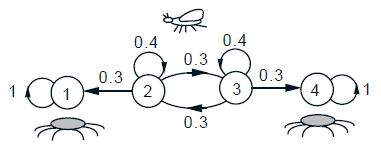
\includegraphics[width=1.53in,height=0.6in]{./media/image1.png}
\end{figure}


%%%%%%%%%%%%%%%%%%%% Figure/Image No: 1 Ends here %%%%%%%%%%%%%%%%%%%%

The transition probabilities  \( p_{ij} \)  must be of course non-negative and sum to one; all of the element of a Markov chain model can be encoded in a transition probability matrix or illustrated in a transition probability graph:\par

 \[  \sum _{j=1}^{m}p_{ij}=1~ \mathrm{\text{for all }}i;~~P= \left[ ~\begin{matrix}
p_{11}  &  p_{12}  &   \cdots   &  p_{1m}\\
p_{21}  &  p_{22}  &   \cdots   &  p_{2m}\\
 \vdots   &   \vdots   &  p_{ij}  &   \vdots \\
p_{m1}  &  p_{m2}  &   \cdots   &  p_{mm}\\
\end{matrix}
 \right]  \] \par

	\item Given a Markov chain model, we can compute the probability of any particular sequence of future states:\par

 \[ P \left( X_{0}=i_{0},X_{1}=i_{1},X_{2}=i_{2}, \ldots ,X_{n}=i_{n} \right) =P \left( X_{0}=i_{0} \right)  \cdot p_{i_{0}i_{1}} \cdot p_{i_{1}i_{2}} \cdots p_{i_{n-1}i_{n}} \] \par

 \[ P \left( X_{1}=i_{1},X_{2}=i_{2}, \ldots ,X_{n}=i_{n} \vert X_{0}=i_{0} \right) =p_{i_{0}i_{1}} \cdot p_{i_{1}i_{2}} \cdots p_{i_{n-1}i_{n}} \] \par

Graphically, a state sequence is similar to a path in the transition probability graph; hence, the probability of such a path (given the initial state) is given by the product of the probabilities associated with the connection traversed by the path.\par

	\item The probability law of the state at some future time, conditioned on the current state called the \textbf{n-step transition probabilities} is defined by:\par

 \[ r_{ij} \left( n \right) =P \left( X_{n}=j \vert X_{0}=i \right)  \] \par

The n-step transition probabilities can be calculated using the following recursion, \textbf{Chapman-Kolmogorov}, equation:\par

 \[ r_{ij} \left( n \right) = \sum _{k=1}^{m}r_{ik} \left( n-1 \right)  \cdot p_{kj};~~\mathrm{for~}n>1;~~\mathrm{\text{starting with }}r_{ij} \left( 1 \right) =p_{ij} \] \par

	\item In addition to the transition matrix, a Markov chain is also characterized by its initial probability distribution which can be represented by a vector  \(  \mu  \)  with entries:\par

 \[  \mu _{i}=P \left( X_{0}=i \right)  \] \par

Using the Chapman-Kolmogorov, it is clear that:\par

 \[ P \left( X_{0}=i \right) = \mu _{i} \] \par

 \[ P \left( X_{1}=j \right) = \sum _{i=1}^{m} \mu _{i} \cdot p_{ij}= \left(  \mu ^{T}P \right) _{j} \] \par

 \[ P \left( X_{2}=j \right) = \sum _{i=1}^{m}P \left( X_{2}=j \vert X_{0}=i \right) = \sum _{i=1}^{m} \mu _{i} \cdot p_{ij}^{2}= \left(  \mu ^{T}P^{2} \right) _{j} \] \par

 \[ P \left( X_{n}=j \right) = \left(  \mu ^{T}P^{n} \right) _{j} \] \par

Theorem: Let $ \{ $ X\textsubscript{0}, X\textsubscript{1}, X\textsubscript{2},...$ \} $  be a Markov chain with m$\ast$ m transition matrix  \( P \) . If the probability distribution of X\textsubscript{0} is given by the 1$\ast$ m row vector  \(  \mu ^{T} \) , then the probability distribution of X\textsubscript{n} is given by the 1$\ast$ m row vector  \(  \mu ^{T}P^{n} \) \textbf{.}\par

 \[ X_{o} \sim  \mu ^{T}  \rightarrow  X_{n} \sim  \mu ^{T}P^{n} \] \par


\end{itemize}\subsection*{Classification of states}
\addcontentsline{toc}{subsection}{Classification of states}
\begin{itemize}
	\item We wish to classify the states of a Markov chain with a focus on the long-term frequency with which they are visited:\par

\begin{itemize}
	\item A state j is \textbf{accessible} from a state i if for some n, the n-stp transition probability  \( r_{ij} \left( n \right)  \)  is positive. \par

	\item A state i is \textbf{recurrent} if for every j that is accessible from i, i also accessible from j. Let A(i) be the set of states that are accessible from i, for all j that belong to A(i), we have that i belongs to A(j). A recurrent state is also called \textbf{absorbing} in the sense that it is infinitely repeated once reached.\par

	\item A state is \textbf{transient} if it is not recurrent. There are states j  A(i) such that i is not accessible from j.\par



%%%%%%%%%%%%%%%%%%%% Figure/Image No: 2 starts here %%%%%%%%%%%%%%%%%%%%


\begin{figure}[H]	\begin{subfigure}		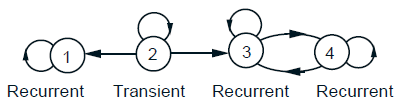
\includegraphics[width=0.45\textwidth]{./media/image2.png}
	\end{subfigure}
~	\begin{subfigure}		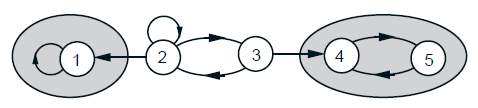
\includegraphics[width=0.45\textwidth]{./media/image3.png}
	\end{subfigure}
~
\end{figure}


%%%%%%%%%%%%%%%%%%%% Figure/Image No: 2 Ends here %%%%%%%%%%%%%%%%%%%%

 \par

	\item If i is a recurrent state, the set of states A(i) form a recurrent class meaning that states in A(i) are all accessible from each other and no state outside A(i) is accessible from them. \par

	\item A Markov chain can be decomposed into one or more recurrent classes plus possibly some transient states.\par


\end{itemize}
	\item Periodicity: a recurrent class is said to be \textbf{periodic} if its states can be grouped in d > 1 disjoint subsets so that all transitions from one subset lead to the next subset. A recurrent class that is not periodic is said to be \textbf{aperiodic}.  \par


\end{itemize}\subsection*{Steady-state behavior}
\addcontentsline{toc}{subsection}{Steady-state behavior}
\begin{itemize}
	\item In Markov chain models, a \textbf{long-term state occupancy} behavior is normally of interested, that is in the \textbf{n-step transition probabilities}  \( r_{ij} \left( n \right)  \)  when n is very large. Sometimes,  \( r_{ij} \left( n \right)  \)  can converge to \textbf{steady-state} values that are independent of the initial state. \par

	\item Consider a Markov chain with a single recurrent class which is aperiodic. Then, the states  \( j \)  are associated with steady-state probabilities  \(  \pi _{j} \)  that have the following properties:\par

\begin{itemize}
	\item  \( \mathop{\lim }_{n \rightarrow \infty}r_{ij} \left( n \right) = \pi _{j}~~\mathrm{\text{for all }}i,j \) \par

	\item  \(  \pi _{j} \)  are the unique solution of the system of equations\par

 \[  \pi _{j}= \sum _{k=1}^{m} \pi _{k}p_{kj}~~~j=1,~2, \ldots , m;    \sum _{k=1}^{m} \pi _{k}=1 \] \par

	\item  \(  \pi _{j}=0 \)  for all transient states j;  \(  \pi _{j}>0 \)  for all recurrent states  \( j \) \par

 \(  \pi _{j} \)  form a probability distribution on the state space, called the stationary distribution of the chain. That means if  \( P \left( X_{0}=j \right) = \pi _{j} \)  with  \( j=1, 2, \ldots , m \)  then  \( P \left( X_{n}=j \right) = \pi _{j} \)  for all  \( n \)  and  \( j \) . Examples on p. 416-423 in Ref. [1] and p. 237-241 in Ref. [2].\par


\end{itemize}
	\item Long-term frequency interpretation\par

Recall that probabilities are often interpreted as relative frequencies in an infinitely long string of independent trials. The steady-state probabilities of a Markov chain admit a similar interpretation as expected state frequencies.\par

For a Markov chain with a single class that is aperiodic, the steady-state probabilities  \(  \pi _{j} \)  satisfy:\par

 \[  \pi _{j}=\mathop{\lim }_{n \rightarrow \infty}\frac{v_{ij} \left( n \right) }{n} \] \par

where  \( v_{ij} \left( n \right)  \)  is the expected value of the number of visits to state j within the first n transitions, starting from state i.  \(  \pi _{j} \)  is the long-term expected fraction of time that the state is equal to j. \par

The expected number of transitions in n transitions that take the state from j to k  \( q_{jk} \left( n \right)  \)  can be calculated as:\par

 \[ \mathop{\lim }_{n \rightarrow \infty}\frac{q_{jk} \left( n \right) }{n}= \pi _{j}p_{jk} \] \par

 \(  \pi _{j}p_{jk} \)  can be viewed as the long-term expected fraction of transitions that move the state from j to k.\par


\end{itemize}\subsection*{Absorption probabilities and expected time to absorption}
\addcontentsline{toc}{subsection}{Absorption probabilities and expected time to absorption}
\begin{itemize}
	\item Aaa\par


\vspace{\baselineskip}

\end{itemize}\subsection*{Random walk models}
\addcontentsline{toc}{subsection}{Random walk models}
\begin{itemize}
	\item Aaa\par


\vspace{\baselineskip}

\end{itemize}\section*{Stoch: Continuous-time Markov chains}
\addcontentsline{toc}{section}{Stoch: Continuous-time Markov chains}
\subsection*{Continuous-time Markov chains}
\addcontentsline{toc}{subsection}{Continuous-time Markov chains}
\begin{itemize}
	\item Aaa\par


\vspace{\baselineskip}

\end{itemize}\subsection*{Brownian motion}
\addcontentsline{toc}{subsection}{Brownian motion}
\begin{itemize}
	\item Aaa\par


\vspace{\baselineskip}

\end{itemize}\subsection*{Birth-Death process}
\addcontentsline{toc}{subsection}{Birth-Death process}
	\item Aaa\par


\vspace{\baselineskip}

\vspace{\baselineskip}
References:\par

\begin{enumerate}
	\item \textbf{\textit{Marcel B. Finan}} Lecture Notes in Actuarial Mathematics – A Probability Course for the Actuaries\par

	\item \textbf{\textit{Dimitri P. Bertsekas $\&$  John N. Tsitsiklis}} Introduction to Probability – Lecture notes MIT 6.041-6.431\par

	\item \textbf{\textit{Anders Tolver}} An introduction to Markov chains\par

	\item \textbf{\textit{Rachel Fewster}} Stochastic processes – Stats 325\par

	\item \textbf{\textit{Andasari}} Stochastic modelling using Python
\end{enumerate}\par



 %%%%%%%%%%%%  Starting New Page here %%%%%%%%%%%%%%

\newpage

\vspace{\baselineskip}\section*{My experiences}
\addcontentsline{toc}{section}{My experiences}
Differential equations\par

\begin{itemize}
	\item Boundary value problem (BVP): a differential equation together with a set of additional constraints, called the boundary conditions.\par

\begin{itemize}
	\item Dirichlet BC: a BC specifies the value of the function itself.\par

	\item Neumann BC: a BC specifies the value of the normal derivative of the function. \par

	\item Cauchy C: a BC has a form of a curve or surface that gives a value to the normal derivative and the function itself. \par


\end{itemize}
	\item Initial value problem (IVP): an ordinary differential equation together with a specified value, called the initial conditions at a given point in the domain of the solution.\par

Partial differential equations (PDE)\par

\begin{itemize}
	\item Hyperbolic, e.g. wave propagation equation\par

	\item Parabolic, e.g. diffusion equation\par

	\item Elliptic, e.g. elasticity and Laplace’s equations\par

	\item Laplace’s equation: a second-order PDE, eg  \( \triangledown ^{2}f=\frac{ \partial ^{2}f}{ \partial x^{2}}+\frac{ \partial ^{2}f}{ \partial y^{2}}=0 \) 
\end{itemize}\par

Finite element method (IBVP)\par

\begin{itemize}
	\item provide the local approximation of the original complex PDE;\par

	\item math term: construct an integral of the inner product of the residual and the weight functions, then set the integral to be zero;\par

	\item simple term: fitting trial functions into the PDE, the residual is the error caused by the trial functions, the weight functions are polynomial approximation functions that project the residual;\par

	\item steady state problems -> a set of algebraic equations -> solved by numerical linear algebra methods;\par

\begin{itemize}
	\item linear systems of equations: Gaussian elimination, iterative method\par

	\item nonlinear systems of equations: Newton-Raphson method\par


\end{itemize}
	\item transient problems -> a set of ordinary differential equations -> solved by numerical integration using standard techniques \par

\begin{itemize}
	\item Newmark\par

	\item Backward/Forward Euler \par

	\item Crank-Nicolson\par

	\item Runge-Kutta.
\end{itemize}
\end{itemize}\par

	\item Step to solve:\par

\begin{itemize}
	\item strong form (PDE) -> (integration by part) -> weak form\par

	\item weak form -> discretization in a finite-dimensional space into piecewise polynomial functions\par

	\item numerical approximation (integration) – Gauss quadrature: implemented on a computer\par


\end{itemize}
	\item Generalized FEM uses local spaces consisting of functions, not necessarily polynomial. Partition of Unity method is used to bond these local spaces together to form the approximating subspace. \par

	\item XFEM: GFEM + PUM + enriching the solution space with discontinuous functions
\end{itemize}\par

Constitutive relations define the dependence of the stress tensor in a body on kinematic variables such as strain tensor or the rate-of-deformation tensor \par

\begin{itemize}
	\item the stress tensor is a mapping of a force vector to a direction vector or a normal vector of a surface that the force is acting on;\par

	\item similar to the strain tensor.
\end{itemize}\par

Smoothed particle hydrodynamics (SPH)\par

\begin{itemize}
	\item an introduction of a kernel function to represent an arbitrary field as a convolution regarding to that kernel function -> any physical quantity of any particle can be obtained by taking the volume integral of the kernel function multiplied by the local value of that quantities of other particles that lie within the range of the kernel (the characteristic radius)\par

	\item the convolution integral is approximated/discretized using a Riemann summation over the particles\par

	\item the kernel functions can be Gaussian function, quintic spline...
\end{itemize}\par


\printbibliography
\end{document}